% !Mode:: "TeX:UTF-8"
% !TEX program  = xelatex
% !BIB program  = biber
\documentclass[AutoFakeBold,AutoFakeSlant,language=chinese,degree=bachelor,zihao=-4]{sustechthesis}
% 1. AutoFakeBold 与 AutoFakeSlant 为伪粗与伪斜,如果本机上有相应粗体与斜体字体,请使用 xeCJK 宏包进行设置,例如:
%   \setCJKmainfont[
%     UprightFont = * Light,
%     BoldFont = * Bold,
%     ItalicFont = Kaiti SC,
%     BoldItalicFont = Kaiti SC Bold,
%   ]{Songti SC}
%
% 2. language=chinese 基于为 ctexart 文类提供的中文排版方案修改,如果使用英文进行论文创作,请使用 language=english 选项。
%
% 3. degree=bachelor 为 sustechthesis 文类提供的本科生毕业论文模板,其他可选项为 master 与 doctor,但是均未实现,如果您对此有兴趣,欢迎 PR。
%
% 4. sustechthesis.cls 文类主要参考自去年完成使命的 sustechthesis.tex,在这一年的时间,作者的 TeX 风格与常用宏包发生许多变化,因为之前的思想为仅提供必要的格式修改相关代码,所以转换为文类形式所进行的修改较少,而近期的风格与常用宏包均体现在以下的例子文件中。
%
% 5. 示例文件均放置于相应目录的 examples 文件夹下,构建自己论文时可暂时保留,用以检索接口与使用方法。
%
% 6. 英文目录需要居中可以使用:\renewcommand{\contentsname}{\centerline{Content}}
%
% 7. LaTeX 中公式编号括号样式及章节关联的方法:https://liam.page/2013/08/23/LaTeX-Formula-Number/

% !Mode:: "TeX:UTF-8"
% !TEX program  = xelatex

% 数学符号与环境
\usepackage{amsmath,amssymb}
  \newcommand{\dd}{\mathrm{d}}
  \newcommand{\RR}{\mathbb{R}}
% 参考文献
\usepackage[style=gb7714-2015]{biblatex}
  \addbibresource{ref.bib}
% 无意义文本
\usepackage{zhlipsum,lipsum}
% 列表环境设置
\usepackage{enumitem}
% 浮动题不越过 \section
\usepackage[section]{placeins}
% 超链接
\usepackage{hyperref}
% 图片,子图,浮动题设置
\usepackage{graphicx,subcaption,float}
% 抄录环境设置,更多有趣例子请命令行输入 `texdoc tcolorbox`
\usepackage{tcolorbox}
  \tcbuselibrary{xparse}
  \DeclareTotalTCBox{\verbbox}{ O{green} v !O{} }%
    {fontupper=\ttfamily,nobeforeafter,tcbox raise base,%
    arc=0pt,outer arc=0pt,top=0pt,bottom=0pt,left=0mm,%
    right=0mm,leftrule=0pt,rightrule=0pt,toprule=0.3mm,%
    bottomrule=0.3mm,boxsep=0.5mm,bottomrule=0.3mm,boxsep=0.5mm,%
    colback=#1!10!white,colframe=#1!50!black,#3}{#2}%
\tcbuselibrary{listings,breakable}
  \newtcbinputlisting{\Python}[2]{
    listing options={language=Python,numbers=left,numberstyle=\tiny,
      breaklines,commentstyle=\color{white!50!black}\textit},
    title=\texttt{#1},listing only,breakable,
    left=6mm,right=6mm,top=2mm,bottom=2mm,listing file={#2}}
% 三线表支持
\usepackage{booktabs}

% LaTeX logo
\usepackage{hologo}
 % 导言区
% !Mode:: "TeX:UTF-8"
% !TEX program  = xelatex
\设置信息{
    % 键 = {{中文值}, {英文值}},
    分类号 = {{}, {}},
    编号 = {{}, {}},
    UDC = {{}, {}},
    密级 = {{}, {}},
    % 仅题目(不含副标题)、系别、专业,支持手动 \\ 换行,不支持自动换行。
    题目 = {{轮腿机器人的设计与控制}, {Design and Control of Bipedal Wheel-legged Robot}},
    % 如无需副标题,删除值内容即可,不可删除键定义。
    副标题 = {{}, {}},
    姓名 = {{赵云天}, {Yuntian Zhao}},
    学号 = {{11811715}, {11811715}},
    系别 = {{机械与能源工程系}, {Department of Mathematics}},
    专业 = {{机器人工程}, {Computatoinal Mathematics}},
    指导老师 = {{贾振中}, {Zhengzhong Jia}},
    时间 = {{2022年05月27日}, {May 7th, 2022}},
    职称 = {{助理教授}, {Assistant Professor}},
}
 % 论文信息
\begin{document}

\中文标题页 % \英文标题页
\中文诚信承诺书 % \英文诚信承诺书
\摘要标题
% !Mode:: "TeX:UTF-8"
% !TEX program  = xelatex
\begin{中文摘要}{轮腿机器人,平衡控制,轨迹跟踪}
  本毕业设计主要设计并制作了一种二轮轮腿机器人,并建立了简化的数学模型,搭建了仿真模型,设计了控制算法并在仿真中进行测试,然后在实物原型机上进行实验。本轮腿机器人拥有6个自由度,其机械设计可靠,电气系统稳定,性能好且易于开发,机器人整体负载较大,可在后期加装传感器、机械臂、用于辅助增强稳定性的动力尾或者涵道发动机。本轮腿机器人所有电机均为准直驱电机,可以实现力控,当前采用PID或者LQR实现轨迹跟踪,后期可结合动力尾、机械臂实现全身控制算法。本轮腿控制系统采用SpeedGoat作为控制器,使用MATLAB Simulink编程,与仿真环境一致,可以实现快速的控制算法实现-仿真测试-实物测试。仿真和实物实验显示,本轮腿的机械、电气和控制系统稳定可靠,且实现了空间轨迹跟踪功能,为后续加装其他负载或实现全身力控算法打下坚实基础。 
\end{中文摘要}


\begin{英文摘要}{Wheel-legged Robot,Balance Control,Trajectory Tracking}
This Undergraduate thesis presents a prototype of a bipedal leg-wheeled robot, with corresponding simplified mathematics and simulation model. The control algorithms are designed and tested in simulation and then transferred to the real-world prototype. This prototype has 6-DOF(Degree of Freedom) with a reliable mechanical design, moreover with a easy-to-develop but powerful digital electric control system. The prototype has a considerable load performance which simplifies further development of adding sensor, powered tail and E-Jets to it in the future. All motors of the prototype are Qausi-Direct Drive(QDD) motors, which are capable of performing force control. Currently, the prototype is controlled with PID or LQR controller to perform trajectory tracking tasks. Further development of Whole-Body Control(WBC) with robotic arm or powered tail installed will be applied to this robot. This robot is controlled by a central compute unit from Speedgoat, which runs the same code of simulation in MATLAB Simulink environment. This has provided a rapid routine for realization of control algorithms from testing in simulation to testing on real-world prototype. The experiment result shows that the mechanical and electric design of the robot is stable and robust, and the robot can perform trajectory tracking tasks well. Generally, it is ready for further development of loaded with other sensors or perform WBC algorithms.
\end{英文摘要}
 % 论文摘要

\目录\clearpage % 目录及换页

\begin{spacing}{1.5}
% !Mode:: "TeX:UTF-8"
% !TEX program  = xelatex
\section{绪论}



\subsection{背景}
21世纪以来,机器人在生产生活中扮演越来越重要的角色。现代机器人是由遥操作演变而来,首先问世的是固定基座的机器人,也就是机械臂,随后才出现了移动机器人\cite{corke2011robotics}。移动机器人运用广泛,包括地面、水下、控制乃至外太空\cite{Siciliano2016handbook}。地面移动机器人则在物流、货物搬运、探索、巡逻等室内外环境有许多用途。

\begin{figure}[h!]
  \centering
  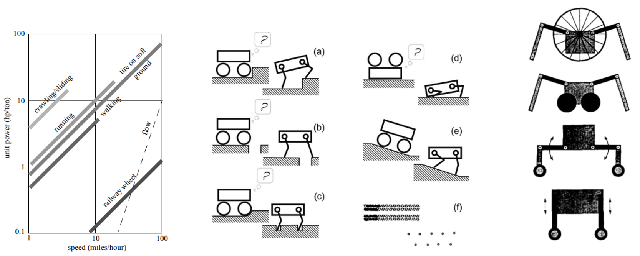
\includegraphics[width=1.0\linewidth]{figures/Sec1/wl.png}
  \caption{
  不同类型的移动(locomotion)效率对比\cite{siegwart2011introduction}(左),与轮式机器人与腿式机器人的通过性对比\cite{siegwart2011introduction}(中),与轮腿独立和轮腿共融的示意图\cite{eiji1993leg}(右)。
  }
  \label{fig:sec1-wl}
   \vspace{6pt}
\end{figure}

主流的地面移动机器人往往是轮式或者腿式,轮式机器人(Wheeled Robot)在平地上效率极高,且其机械结构简单,可靠性好,易于控制,率先得到了快速的发展与广泛的运用。结合一些感知与规划的算法,轮式机器人已经广泛运用在生产生活中,如无人工厂AGV\cite{Siciliano2016handbook}\cite{khatib2016springer}(Auto Guided Vehicle,自动引导车辆),无人码头的集装箱运转车辆\cite{Qingdaoport}和在家庭中常见的扫地机器人,甚至近些年来得以迅速发展的无人驾驶车辆。但面对一些复杂的非结构化环境下的任务,如在具有楼梯的建筑物内巡检,或在废墟中救援等等,传统的轮式移动机器人已经难以满足实际应用的需求。这些场景或者是为人类生产生活所设计的,如梯子、楼梯,有些则对于人类也充满挑战,如废墟等等。轮式机器人需要在平整的地面上才能发挥出速度快、效率高的优势,但在这些场景则会卡在障碍物中或无法上下楼梯,因而无法完成任务(如图\ref{fig:sec1-wl}中所示)。

而腿式机器人(Legged Robot)具备在复杂非结构化环境中更好的机动性和适应性,尤其是双足腿式机器人(Biped Legged Robot),其落地点可以在一定范围内选取,且腿可以实现一种类似于主动悬挂的效果\cite{Raibert1984walkingrobots}(如图\ref{fig:sec1-wl}中所示),非常适合在为人类设计的环境中工作\cite{Yamaguchi1997humanoid}。但腿式机器人移动速度慢,能量消耗高(如图\ref{fig:sec1-wl}左所示),且双足机器人控制困难。相比于轮式机器人,腿式机器人须要拥有更多自由度,且关节扭矩大,因此对驱动系统和机械设计提出很高要求。双足机器人的运动控制须考虑其平衡,且须规划落脚点,然后控制各个关节,规划及运动控制难度和复杂度都远超轮式机器人,且在运动速度远不及轮式机器人的情况下,消耗的能源也远超轮式机器人。

双足轮腿机器人(Bipedal Leg-wheeled Robot,以下简称轮腿机器人)结合了轮式机器人的高速高效性和腿式机器人对复杂地形的适应性强的特点,增大机器人作业范围和环境适应性,这些机器人在平地上使用轮子移动,遇到障碍物时则跳过或跨过障碍物(如图\ref{fig:sec1-wl}右所示)。轮腿共融机器人的两侧的腿可以独立改变长度,使得机器人通过性、机动性更好,能在狭小空间中运动,转弯时保持高速,还能在不平整地面保持平衡。当然,轮腿机器人也结合了轮式和腿式的其他特点,其控制复杂度比轮式高,但却不需要像腿式机器人一样需要规划落脚点和步态,因此难度比腿式机器人低。正因为结合了轮式与腿式的优点,轮腿机器人近年来得到了广泛的发展。

\subsection{国内外研究现状}

国外的Boston Dynamics的Handle机器人(图\ref{fig:sec1-Handle})在物流、仓储方面表现出令人惊叹的稳定性、灵活性和效率,但是Boston Dynamics并未发表论文公开其背后的机械设计及控制算法等。据开源资料披露,其移动速度可达24km/h,远超过该公司的双足机器人Atlas 5km/h的速度。Handle物流机器人拥有一个巨大的“动力尾”,笔者推测其液压动力系统和电池等安装在其中。根据Boston Dynamics展示的视频信息,Handle机器人在加减速和拿起货物的时候,“动力尾”会主动运动以辅助机器人保持平很,以提升机器人的整体性能。

\begin{figure}[h!]
  \centering
  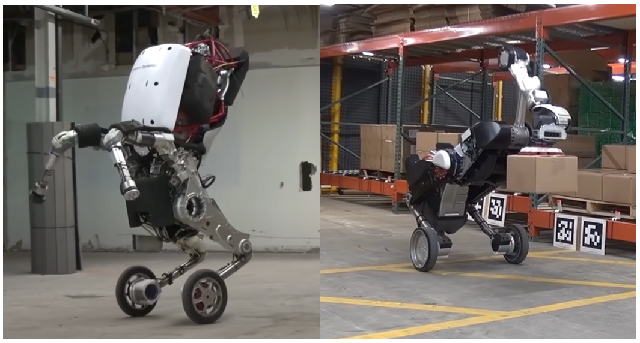
\includegraphics[width=0.5\linewidth]{figures/Sec1/Handle.png}
  \caption{
  Boston Dynamics的第一代\cite{introducinghandle}(左)和第二代\cite{handle4logistics}(右)Handle机器人
  }
  \label{fig:sec1-Handle}
   \vspace{6pt}
\end{figure}

ETH的Ascento(图\ref{fig:sec1-Ascento})机器人发表了论文,介绍了其使用场景、机械设计和控制算法,其主要应用场景为探索、监控、巡查,其腿部仅有一个自由度,并经过拓扑优化设计四杆机构,使得电机可以控制机器人质心近似上下移动,从而实现跳跃功能。其跳跃功能是为了上楼梯涉及的,后来Ascento机器人被开发用于巡逻与探索,且推出专业版(图\ref{fig:sec1-AscentoPizza})。普通的Ascento机器人其鲜有搭载负载的场景,考虑到其轮腿设计,安装负载时必须使其质心与机器人与地面接触点连线竖直,如图\ref{fig:sec1-AscentoPizza}所示。Ascento专业版机器人采用了悬吊的方式装载重物,但其没有发表论文或公开资料,因此实际性能并未可知。Ascento机器人的2019年iCRA\cite{klemm2019ascento}论文主要提出了基于多个参数插值的LQR平衡方式,同时通过调试的方式实现了摔倒-站立和定高度跳跃,然后在2020RAL\cite{klemm2020lqr}期刊中运用了全身力控,进一步增强了稳定性和抗扰能力。

\begin{figure}
  \centering
  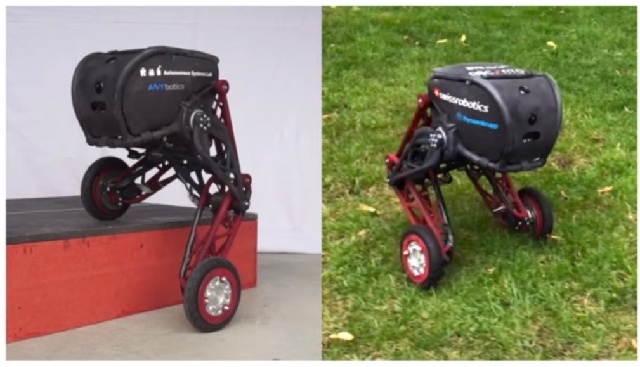
\includegraphics[width=0.5\linewidth]{figures/Sec1/Ascento.png}
  \caption{
  ETH的Ascento机器人\cite{klemm2019ascento} \cite{klemm2020lqr}
  }
  \label{fig:sec1-Ascento}
   \vspace{6pt}
\end{figure}

\begin{figure}
  \centering
  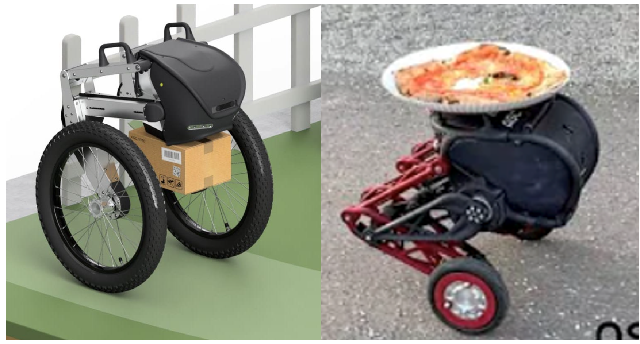
\includegraphics[width=0.5\linewidth]{figures/Sec1/AscentoPizza.png}
  \caption{
  Ascento专业版\cite{ascentopro}机器人运送货物时,将货物吊装在机体下方(左),Ascento机器人运送货物时,需调整货物位置(右)
  }
  \label{fig:sec1-AscentoPizza}
   \vspace{6pt}
\end{figure}


哈尔滨工业大学的WLR机器人(图\ref{fig:sec1-HITWRL})尺寸与Handle机器人接近,其同样采用液压驱动 ,使用金属3D打印作为液压动力输送管道,但其动力源是外置的,且机器人尺寸较大,因此并不适用于室内环境进行家庭服务等工作。

\begin{figure}[h!]
  \centering
  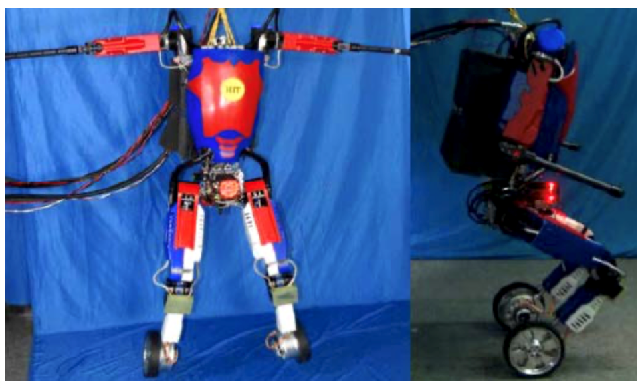
\includegraphics[width=0.5\linewidth]{figures/Sec1/HITWRL.png}
  \caption{
  哈尔滨工业大学的WLR机器人\cite{li2018design}
  }
  \label{fig:sec1-HITWRL}
   \vspace{6pt}
\end{figure}

腾讯的Ollie机器人(图\ref{fig:sec1-Ollie})采用了五杆机构设计的腿部结构,与传统的双足足式机器人有较大差别。五杆机构属于并联机构,因此可以获得扭矩叠加的效果,从而优化跳跃表现,但并联机构也带来了解算复杂、工作空间小的缺点。此外,Ollie机器人还设计有一个安装了万向轮的尾巴,类似于Handle物流机器人的动力尾,在Ollie展示其“翻跟斗”的能力时,尾巴很好的辅助其完成旋转一周的动作,但据Ollie披露的视频显示,尾巴仅在此发挥作用,其余时间均收起,与身体保持固连的状态。

\begin{figure}[h!]
  \centering
  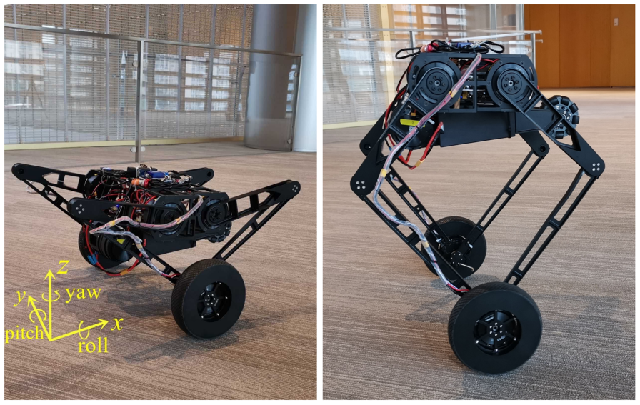
\includegraphics[width=0.5\linewidth]{figures/Sec1/Ollie.png}
  \caption{
  腾讯的Ollie机器人\cite{wang2021balance}
  }
  \label{fig:sec1-Ollie}
   \vspace{6pt}
\end{figure}

南方科技大学的哪吒(NeZha)机器人(图\ref{fig:sec1-sr600nezha})在控制上体现出强大的稳定性与鲁棒性,并首次提出了轮腿机器人跳跃的综合规划与控制策略\cite{chen2020underactuated},并在仿真中得到了验证。

\begin{figure}[h!]
  \centering
  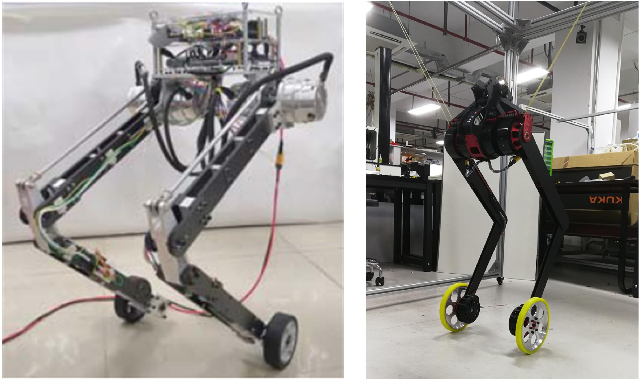
\includegraphics[width=0.5\linewidth]{figures/Sec1/sr600nezha.png}
  \caption{
  哈尔滨工业大学(深圳)的SR600机器人\cite{zhang2020sr600}(左)和南方科技大学的哪吒机器人(右)
  }
  \label{fig:sec1-sr600nezha}
   \vspace{6pt}
\end{figure}

哈尔滨工业大学(深圳)的SR600机器人(图\ref{fig:sec1-sr600nezha})采用了QDD\cite{wensing2017proprioceptive}(Qausi-Direct Drive,准直驱)的膝关节和髋关节电机,但采用有刷电机作为轮子驱动器,且经过减速箱、弹性联轴器与锥齿轮传动,无法实现力透传,且其QDD电机减速比过大。该机器人实现了静态平衡\cite{zhang2019system},并在仿真中实现了变高度平衡\cite{liu2019dynamic}。

\subsection{研究内容和系统框架}
本毕业设计希望能实现设计搭建类似于Ascento机器人的样机。Ascento使用单自由度四连杆机构,通过优化杆长实现近似上下运动。与之不同的是,本毕设使用双电机设计,从而在运送货物时无须调整其位置,使得整体布局更接近SR600机器人的设计。本毕设的目标场景是,在为人类设计的室内环境中,机器人能前往该环境的所有地点。相比于Handle机器人和WLR机器人,本毕设采用的方案成本更低、更易于实现,可以推广到家庭、餐馆、医院服务等无须大载重,但对机器人尺寸、灵活度要求较高的场景。Ascento虽然实现了全身控制\cite{klemm2020lqr},但其自由度偏少,而SR600虽然使用了QDD电机,但其减速比过高(60:1,甚至不符合文献\cite{wensing2017proprioceptive}中要求的减速比不大于36:1),且轮子电机及相关传动、减速无法实现力控。本毕业设计的创新点在于,全部采用减速比在10:1之内的QDD电机,实现效果更好的QDD力控,因而可以为后续基于此平台实现全身控制及跳跃做准备。

\begin{figure}[t!]
  \centering
  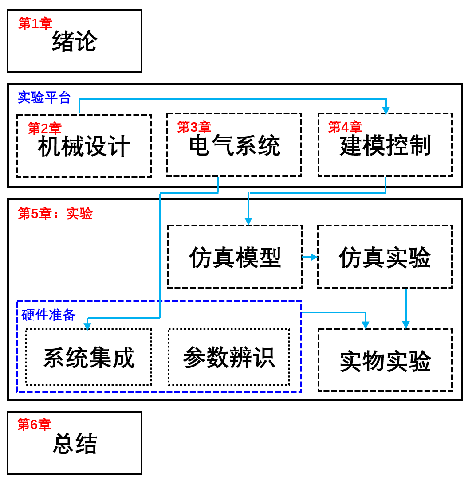
\includegraphics[width=0.7\linewidth]{figures/Sec1/frame1.png}
  \caption{
  论文各章节主要内容
  }
  \label{fig:sec1-frame1}
   \vspace{4pt}
\end{figure}

本毕设将先分析将要设计的轮腿机器人的结构并基于此展开机械设计,然后将QDD电机和驱动器、电池、计算平台运用并布置其中。根据机械设计,本毕设将对机器人进行等效、简化的建模。将建立运动学模型一遍调试及是实现简单的控制,建立动力学模型以了解系统特性,并依次设计若干控制器。本毕设将首先设计简单的控制器,以验证整套硬件系统,然后更换为复杂但效果更好的控制器。同时会根据机械设计与建模结果搭建仿真模型,并在仿真中测试控制器,进行仿真实验。为将上述控制器迁移到实物中,需要进行硬件准备。本毕设将根据电气系统中选用的各部件进行联调,实现系统集成的效果,然后对机器人本体进行参数辨识,以更正仿真模型中使用CAD(Computer Assistant Design,计算机辅助设计)模型估算的各种误差。最终,通过仿真验证的控制器将会迁移到通过硬件准备的实物上,进行实物实验。

本毕设论文的组织形式如图\ref{fig:sec1-frame1}所示,考虑到本毕设的目的是设计与制作实验平台,并运用控制算法,因此第二章、第三章和第四章分别从机械设计、电气系统和建模控制的角度介绍。为验证本毕设设计制作的轮腿机器人的实际效果,需要进行实验,包括仿真实验和实物原型机实验。在进行仿真实验之前,需要进行仿真模型搭建,而进行实物实验之前,需要对硬件平台进行准备,如电气系统集成和参数辨识等。

本毕业论文的包括的主要内容及主要的贡献点如图\ref{fig:sec1-frame2}所示,也分别对应每个章节的相应内容。

\begin{figure}[h!]
  \centering
  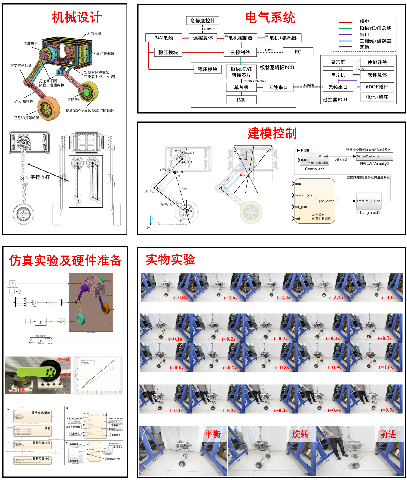
\includegraphics[width=0.9\linewidth]{figures/Sec1/frame2.1.png}
  \caption{
  论文总体框图
  }
  \label{fig:sec1-frame2}
   \vspace{4pt}
\end{figure}

\subsection{本章小结}
本章中,介绍了轮腿机器人结合了轮式机器人和腿式机器人的优点,以及国内外的相关研究现状。然后介绍了本文的研究内容和研究框架,最终本毕业设计的最终实物如图\ref{fig:sec1-result}所示。

\begin{figure}[t]
  \centering
  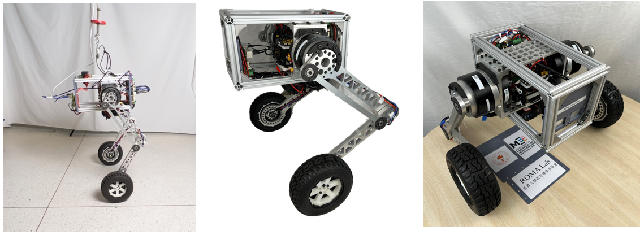
\includegraphics[width=1.0\linewidth]{figures/Sec1/result.png}
  \caption{
  本毕业设计最终实现的轮腿机器人原型机示意图
  }
  \label{fig:sec1-result}
   \vspace{4pt}
\end{figure}\clearpage
% !Mode:: "TeX:UTF-8"
% !TEX program  = xelatex
\section{机械设计}

\subsection{引言}

机器人的机械设计是由机器人的目标任务决定,由电气部件选择、加工方式、工作场景等条件所约束,以突出创新点、优化系统整体性能为目标。本章将会先介绍本机器人的目标任务,以及上述的约束条件和创新点,然后会围绕这些内容,分成以下三个部分,依次展开机械设计的具体内容。首先是机器人的结构设计,包括机器人的自由度、驱动模块选择,驱动器的布置与传动方式,和机器人的活动范围与限位的设计。然后介绍了具体的机械设计,包括结构件的设计与强度校核,关节设计与连接件的选择。最后介绍了与电气系统相关的机械设计,具体是电气零部件的布置与线缆的布置与收纳。
% 机器人的实拍图如图图所示。

% \begin{figure}
%   \centering
%   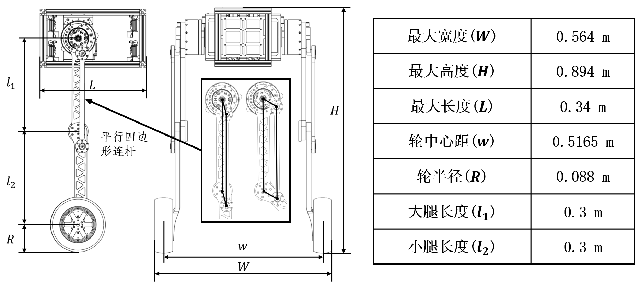
\includegraphics[width=0.4\linewidth]{figures/Sec2/dim.png}
%   \caption{
%   轮腿机器人的外形尺寸与主要杆件长度示意图。其中膝关节通过平行四边形连杆实现了远端驱动\cite{spong2006robot},减小了腿部的表征惯量(apparent inertia)。
%   }
%   \label{fig:sec2-dim}
%   \vspace{6pt}
% \end{figure}

% \begin{figure}
%   \centering
%   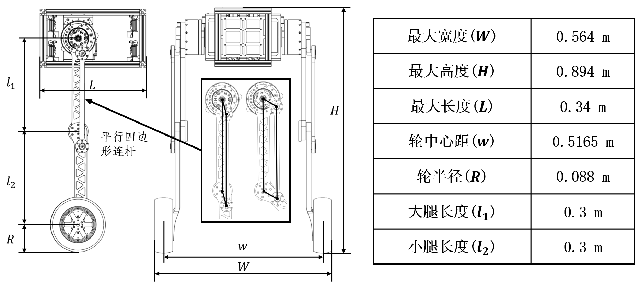
\includegraphics[width=0.4\linewidth]{figures/Sec2/dim.png}
%   \caption{
%   轮腿机器人的外形尺寸与主要杆件长度示意图。其中膝关节通过平行四边形连杆实现了远端驱动\cite{spong2006robot},减小了腿部的表征惯量(apparent inertia)。
%   }
%   \label{fig:sec2-dim}
%   \vspace{6pt}
% \end{figure}

如绪论中所述,本轮腿机器人的目标任务是在为人类设计的生活工作环境中辅助人类,例如物流、家务、看护等。考虑到某些任务并无法使用单独的轮腿来实现,如物流相关的任务需要机械臂以实现抓取移动、激光雷达和深度相机以实现物体识别和环境感知,因此本毕业设计的轮腿机器人主要是机器人底盘,负责具体实现基础的平衡与轨迹跟踪,后续相关功能如任务规划、避障或机械臂抓取等则可以在此平台基础上开发。在适合人类生活与工作的空间,最佳选择是与人类体型、体重相若的仿人机器人,但如绪论中所分析,其存在相当多的技术难点。因此轮腿机器人的设计目标是,身高与人类身高的一半相仿,尺寸与人类体型相近,且质量尽可能轻以提高机器人运动性能,增强续航。基于以上几点,轮腿机器人最终设计出来的尺寸如图\ref{fig:sec2-dim}所示。

\begin{figure}[h!]
  \centering
  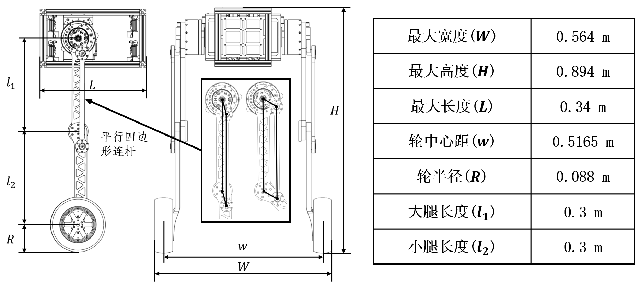
\includegraphics[width=0.9\linewidth]{figures/Sec2/dim.png}
  \caption{
  轮腿机器人的外形尺寸与主要杆件长度示意图。其中膝关节通过平行四边形连杆实现了远端驱动\cite{spong2006robot},减小了腿部的表征惯量(apparent inertia)。
  }
  \label{fig:sec2-dim}
   \vspace{6pt}
\end{figure}

考虑到机器人主要在室内场景工作,因此无需特别防水防尘设计。考虑到仅仅是原型机打样及,加工方式及预算较为宽裕,但需要频繁测试迭代,因此加工周期是重要考量因素,除了强度与精度要求高的结构件与配合使用CNC加工外,铝型材等预制件被广泛采用;此外,各种3D打印件也被使用在不同场景,如对韧性需求高的限位件使用尼龙3D打印,电机控制器、编码器的安装使用光固化或热熔沉积3D打印等等。

\begin{figure}
  \centering
  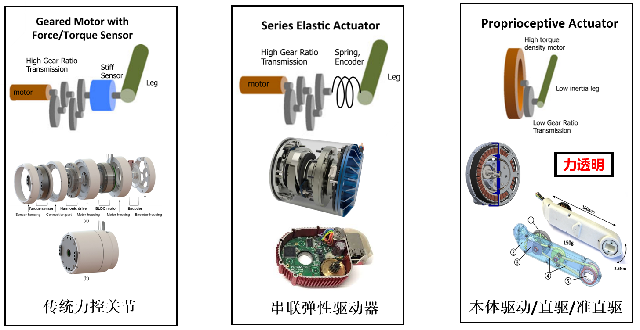
\includegraphics[width=0.7\linewidth]{figures/Sec2/force.png}
  \caption{
  轮腿机器人所使用的驱动器(电机),从左到右分别是胯部电机RMD-X8,定制膝盖电机和轮子电机AK-80-6.
  }
  \label{fig:sec2-force}
   \vspace{6pt}
\end{figure}

驱动系统是机器人运动的核心。考虑到液压驱动系统的难度高、体积大,不适合本毕业设计所期望的工况,因此本轮腿机器人计划采用电机驱动。而考虑到机器人后续的相关控制算法的应用,驱动电机需要具有力控功能。当前实现力控的方案一共有如图\ref{fig:sec2-force}所示的三种方案:传统力控关节,使用高减速比电机和力传感器实现,控制带宽高但无反驱能力,受到较大外力冲击易损坏传感器和减速器,应用于在KUKA iiwa\cite{bischoff2010kuka}和Kinova机械臂中;串联弹性驱动器(SEA)\cite{pratt1995series}使用双编码器测量弹性体形变间接测量力矩,具有柔性储能结构,耐受冲击,但高频力矩性能相应较弱;准直驱方案\cite{seok2012actuator}\cite{wensing2017proprioceptive}由于低减速比因此力透明,通过驱动器电流环直接进行力控,可以实现高频相应且抗冲击能力强,但输出扭矩密度不足。在三种方案间权衡,本毕业设计决定采用基于本体感知的准直驱电机作为力控方案,类似的方案被用在了麻省理工学院的Mini Cheetah机械狗\cite{katz2019mini}上,以及Agility Robotics推出的本体驱动双足机器人Cassie\cite{apgar2018fast-cassie}与Digit上。

\begin{figure}
  \centering
  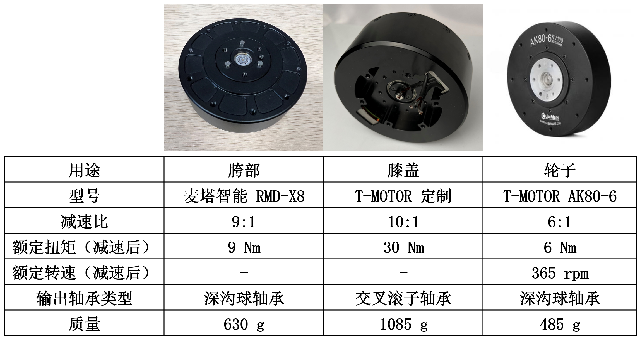
\includegraphics[width=0.9\linewidth]{figures/Sec2/motors.png}
  \caption{
  常见的三种力控机器人关节电机方案示意。
  }
  \label{fig:sec2-motors}
   \vspace{6pt}
\end{figure}

本轮腿机器人的创新点与电气部件中的驱动器(电动机)紧密相关,并且考虑到轮腿机器人膝关节需求扭矩大,市场上可供选择的驱动器种类少的限制条件,因此也需要根据实际驱动器选型调整轮腿的关键尺寸参数,如大腿和小腿的长度等等。如绪论中所述,本轮腿机器人的创新点之一在于使用准直驱实现所有驱动器的力矩控制。准直驱在绪论中已经有过叙述,在此不再赘述。考虑到机器人的膝关节扭矩最大,且准直驱要求电机减速比不能过高,因此最终膝关节选择了T-Motor定制电机(如图\ref{fig:sec2-motors}),具体参数在电气系统章节给出。该电机持续扭矩输出为30Nm(10:1减速之后),根据机器人预估质量进行静力学校核,并乘以安全系数之后,选定机器人的大腿及小腿长度,如上文图\ref{fig:sec2-dim}所示。


\subsection{轮腿机器人的结构设计}
如绪论所述,轮腿机器人的“腿”的部分的自由度有诸多选择,同时也有多种驱动器驱动形式,如Ascento机器人使用单个电机,但通过拓扑优化杆长,使用四杆机构实现上下运动;腾讯的Ollie机器人使用五杆并联机构,虽然活动范围小,但是单个电机所需扭矩并不是很大;而Handle机器人则拥有扭矩巨大的液压驱动器,因此可以使用与人或动物的腿最为相近的串联设计。在后续的子章节中,将会首先介绍自由度及驱动模块,然后是与相关的优化:远端驱动及连杆传动,最后介绍了轮腿机器人的活动范围(工作空间),以及限位的设计。

\subsubsection{自由度及驱动模块}
上一部分中,本毕设对比了几种电机布置形式与自由度的选择。考虑到轮腿机器人的用途,后续可能加装机械臂用来搬运物体,或动力尾以增强平衡能力与机动性,机器人的躯干部分(如图\ref{fig:sec2-dof-parts})的质心会经常改变。为了使机器人在质心改变之后仍能再视觉上保持躯干的竖直状态,这一点对于激光雷达、深度相机进行环境感知提供了便利和持续一致的视野,我们选择使用2自由度的腿部设计。否则如果采用单自由度仅能变高度的设计,则需要在改变负载时精心调整负载位置,或使机器人整体在一个倾斜的角度平衡,前者是运送货物时难以做到的,而后者则是感知时不希望看到的。
综上所述,本毕设提出的机器人将会有每条腿2个自由度,轮子1个自由度,总共6个自由度的设计,如图\ref{fig:sec2-dof-parts}所示。在这里需要说明的是,使用并联的5杆机构同样可以实现上述需求,并且并联机构能够使电机合力更大,但是考虑到结构的简单性,并考虑到已有性能较强的电机,本毕设使用的是串联构型。

\begin{figure}
  \centering
  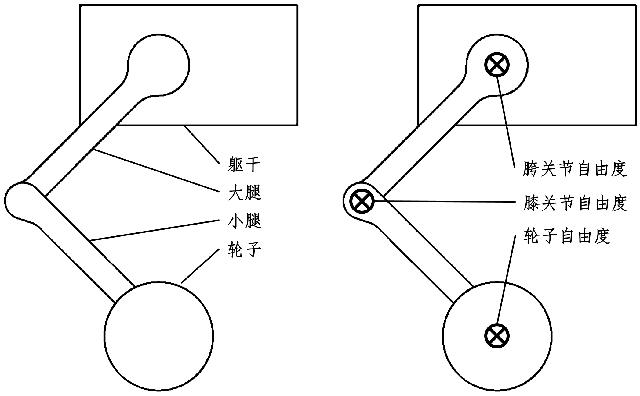
\includegraphics[width=0.75\linewidth]{figures/Sec2/dof-parts.png}
  \caption{
  左图:轮腿机器人可以分成躯干、大腿、小腿、轮子几个部分,之后也会用这些名称来代指。右图:轮腿机器人的自由度分布,分别是轮子、膝盖、胯部。
  }
  \label{fig:sec2-dof-parts}
   \vspace{7pt}
\end{figure}

在本章的引言中,膝关节的驱动模块已经被粗略介绍过了,与其他机器人驱动器的具体技术细节一起,将在电气系统章节给出。这里的选型依据是综合考量输出扭矩、最大转速、减速器齿隙、输出配合然后决定的。值得注意的是,电磁电动机的扭矩与体积有如下固定的上限关系如公式\ref{eq:motor-tau-vol}\cite{hughes2006electric}所示,其中$D^2L$与体积成正比。
\begin{equation}
    T = (\bar{A}\bar{B})\times (\pi DL) \times D / 2 = \frac{\pi}{2} (\bar{A}\bar{B}) D^2 L
    \label{eq:motor-tau-vol}
\end{equation}
而减速器的加入可以增加电机的输出扭矩,但也会减少力的透明传输特性与反驱能力,因此减速比的选择也是重要的考量因素。
膝关节驱动器具有特殊性,这里不再赘述。轮子电机选用T-Motor的AK80-6(如图\ref{fig:sec2-motors}),考虑到轮子并无需提供很大扭矩,但需要有较快的转速,因此选用尺寸、功率合适而减速比为6:1的该型号电机。由于胯部电机安装在躯干上,同时负责驱动躯干的旋转,选择的侧重点则是自重和扭矩,因此选择了尺寸、功率合适的9:1减速比的麦塔智能的RMD-X8电机(如图\ref{fig:sec2-motors})。这两个电机的输出配合、安装方式、常见工况将在下一子章节中详细展开。膝盖电机在上文已经介绍过,也将在电气章节详细展开。

\subsubsection{远端驱动及连杆传动}
% 机器人整体结构设计图及平行连杆结构
在确定了自由度与驱动器之后,驱动器的位置布置与传动方式的选择将在本节讨论。考虑到本轮腿属于验证原型机性质,驱动方式尽量从简,且轮子和胯部电机本身就是带有减速器的QDD电机,因此它们通过合适的关节和连接件直接驱动对应的轮毂和大腿杆件。而考虑到膝关节电机质量较大,为减少系统建模与控制难度,减少表征惯量,考虑了运动范围和扭矩,将电机布置在远端(躯干位置,与胯部电机同心),采用平行四边形连杆机构传动,具体如图\ref{fig:sec2-dim}所示。值得注意的是,考虑到运动范围与轮腿机器人常见位姿,以及小腿的加工复杂度,选择了当前平行四边形的短杆长度。这样在增加限位之后(在下一节会介绍限位),连杆不会达到奇异位置,而膝关节驱动器便可等效安装在膝关节位置而不是远端。在后文的建模和控制章节中,运动学也可以进行等效,动力学也可以进行简化。

\subsubsection{活动范围及限位设计}
对于串联结构的腿式机器人,膝盖弯曲方向也是应当考虑的。人类的膝盖是向前弯曲的,而马、鸵鸟等动物的趾骨也是腿的一部分,因此可以观察到向后弯曲的腿。笔者认为,对于无需通过步态实现移动的轮腿机器人,由于大腿与小腿的长度相等,因此膝盖的方向选择更多需要考虑实际工作情况。考虑到后续可能在轮腿机器人上安装机械臂,例如需要靠近桌子使用机械臂夹取桌上物品(如图\ref{fig:sec2-table}所示),因此选择膝盖后弯的形式。和在绪论中介绍的一样,Handle机器人(图\ref{fig:sec1-Handle})和Ascento机器人(图\ref{fig:sec1-Ascento})也都采用膝盖后弯的形式。

\begin{figure}[h!]
  \centering
  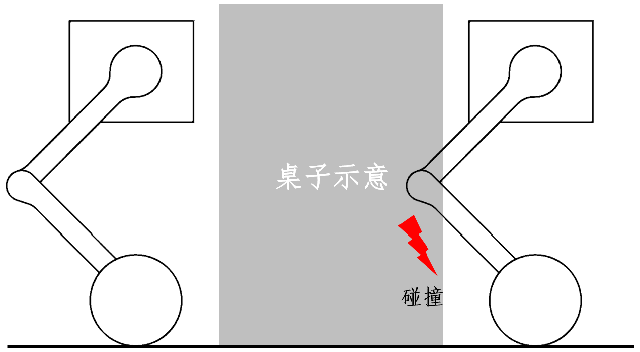
\includegraphics[width=0.75\linewidth]{figures/Sec2/table.png}
  \caption{
  如图所示,如果机器人需要靠近桌子使用机械臂夹取桌子上的物体,则膝盖向后完全的形式比膝盖向前弯曲的形式有更大概率免于碰撞。
  }
  \label{fig:sec2-table}
   \vspace{5pt}
\end{figure}

上一章节有关连杆设计的部分,对于膝盖前弯和后弯而言都可以使用相同的参数,区别在于连杆的布置位置朝前或朝后。在确定了膝盖弯曲的方向之后,也便可以定义机器人的前后、左右、上下,也就是矢状面、冠状面、横断面,如图\ref{fig:sec2-3lim}所示。因此膝盖限位可以直接设计在连杆上,使用尼龙3D打印,以兼顾刚性、韧性和弹性。在后续实验章节的系统集成子章节中,将会介绍基于状态机的电流及位置限制器,以确保电机不会撞到限位或以较大扭矩挤压限位,因此这里的机械限位除了作为最后一道安全限位措施外,主要实现了机器人下电状态下支撑机器人和绝对位置编码器校准的作用。在轮腿机器人的膝盖电机在静能状态下,电机完全不输出扭矩,限位件支撑机器人到最低高度,轮子和膝盖保护件与地面接触,支撑机器人,膝盖保护件采用硬度较高且较光滑的尼龙3D打印件制作,实现了双轮差速车的效果。

\begin{figure}
  \centering
  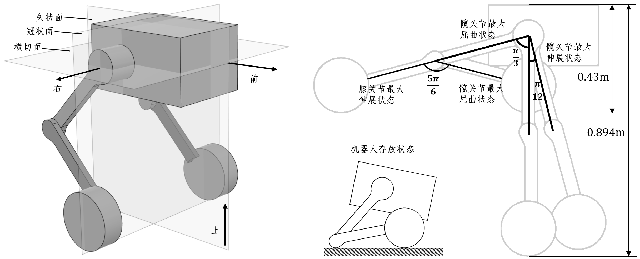
\includegraphics[width=1.0\linewidth]{figures/Sec2/3lim.png}
  \caption{
  左图:轮腿机器人的矢状面、冠状面和横切面,以及相应的前、右、上方向。右图:机器人的膝关节和髋关节的限位大小及机器人平衡时的最大最小高度,左下则是当机器人关闭电源时,凭借关节限位与膝盖支撑件保持摆放状态。
  }
  \label{fig:sec2-3lim}
   \vspace{7pt}
\end{figure}


胯部的限位件的设计考虑了在整个机器人可变高度的范围内,需要通过胯部电机和膝盖电机配合以确保机器人躯干竖直向上。因此胯部限位件在某一方向限制胯部电机的运动幅度与膝盖电机的运动幅度相关,而在另一方向则选择了一个较小的值,以实现如前文所述的在一定范围内调整重心的需求。
膝盖限位件需要限制膝盖电机的运动范围在180°以内,以防止连杆机构奇异,但实际上接近竖直的状态连杆会对限位件产生巨大的压力而导致形变,使连杆系统处于奇异状态,因此在本原型机中,将膝盖电机的运动范围限制在以完全折叠为0°的30°到180°范围内。根据前文所述,胯部限位件将胯部电机的活动范围限制在以竖直位置为0°的-75°到15°的范围内,如图\ref{fig:sec2-3lim}所示。

\subsection{轮腿机器人的机械设计}
在本子章节中,将会介绍轮腿机器人的具体设计,包括CNC结构件的设计、减重与强度校核,不同3D打印件的用途与设计,然后介绍了关节和连接件的设计与配合。这些机械设计的图纸与3D打印零件的示意图会附在附录中。

\subsubsection{结构件设计及强度校核}
在前面的子章节中,轮腿机器人的大腿和小腿长度都已经确定了,同时考虑到远端驱动的连杆设计,小腿的宽度也已经确定。为了追求视觉的一致性,大腿的宽度与小腿选择一致。在此基础上,厚度与镂空方式将根据经验选择,然后再通过有限元仿真进行强度校核。本轮腿设计使用的CAD软件使Autodesk公司的Fusion 360,内置静力学仿真,根据机器人的典型重量和重力、宽度产生的扭矩对小腿和大腿的目前设计进行了强度校核,如图\ref{fig:sec2-simu}所示。

\begin{figure}
  \centering
  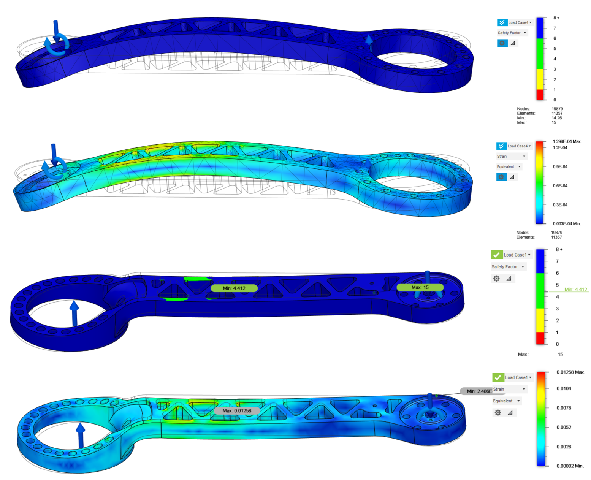
\includegraphics[width=0.85\linewidth]{figures/Sec2/simu.png}
  \caption{
  上2张图:大腿杆件在有限元仿真中的静力学负载工况下的安全系数和应变。值得注意的是图中所展示的形变是夸张的展示形变的趋势而远非实际情况。下2张图:小腿杆件在有限元仿真中的静力学负载工况下的安全系数和应变。
  }
  \label{fig:sec2-simu}
   \vspace{5pt}
\end{figure}

值得注意的是,上述的扭矩和重力在设计关节和连接件如轴承的选用时,也将同样纳入考量范围。

\begin{figure}[h!]
  \centering
  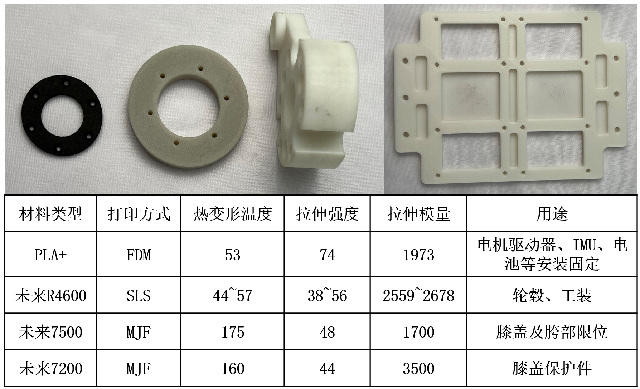
\includegraphics[width=0.85\linewidth]{figures/Sec2/3dp.png}
  \caption{
  上图从左到右依次是未来7500,未来7200,未来R4600及PLA+,下图则是这些3D打印材料的机械性能及使用用途。
  }
  \label{fig:sec2-3dp}
   \vspace{6pt}
\end{figure}

所有3D打印件的材料、用于、机械性能如图\ref{fig:sec2-3dp}所示,上文已经提到过膝盖支撑3D打印件,这里不再赘述。膝盖限位件的设计与远端驱动的连杆在到达限位的位置进行平面的配合,如图\ref{fig:sec2-2lim}所示,而胯部限位件则采用两个圆弧面与胯部电机的输出盘配合以起到限位的效果,如图\ref{fig:sec2-2lim}所示。在下一节中,将会介绍包括电机输出在内的连接件,而本轮腿机器人的轮胎和胎皮都采用RC现成产品,而轮毂则由3D打印制成。关于轮毂的设计的细节将在下一节中详细展开。电机编码器、电机驱动器、IMU、电池等机电部件也广泛使用3D打印配件固定,和躯干上的铝型材保护框架,都将在下一子章节介绍。

\begin{figure}
  \centering
  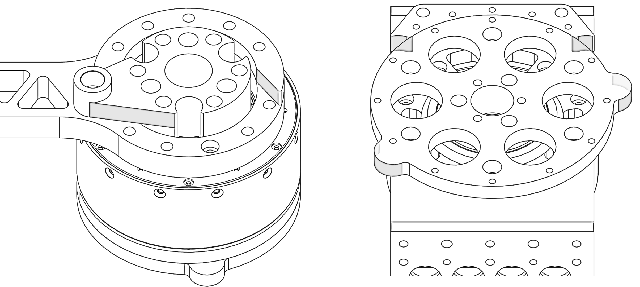
\includegraphics[width=0.85\linewidth]{figures/Sec2/2lim.png}
  \caption{
  膝盖和胯部的限位设计。
  }
  \label{fig:sec2-2lim}
   \vspace{6pt}
\end{figure}

\subsubsection{关节设计与连接件选择}
在本节中,主要包括轮腿的关节,及关节的连接件,如膝关节使用的交叉滚子轴承,各电机输出盘的配合,连杆的轴承选择与配合等等。
如上文所述,轮子电机选用的时T-Motor的AK80-6,其具有内置的行星减速箱,输出轴为一个深沟球轴承。为了优化电机安装厚度通过设计轮毂使得轮胎中心过电机输出的深沟球轴承,从而使该轴承主要承受因重力而产生的径向力,在轮腿机器人转弯时需要承受较小的轴向力。而该设计使得轴承无需承受转矩,从而无需额外轴承及配合,如图\ref{fig:sec2-mech}所示,使得轮子设计更为紧凑。考虑到轮毂的加工难度和快速打样的需求,采用光固化的3D打印加工,但是其表面硬度不足,与直径较小销进行配合后,当电机输出较大扭矩时,容易使轮毂形变从而导致背隙。因此本设计采用多颗直径较大的塞达螺丝与轮毂配合的形式。

\begin{figure}
  \centering
  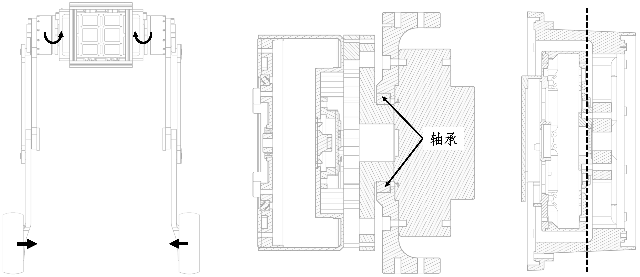
\includegraphics[width=0.85\linewidth]{figures/Sec2/mech.png}
  \caption{
  左图:当轮胎受到同向的力时,将在胯部产生巨大扭矩。中图:胯部的双轴承设计,分别是图中所示轴承与电机输出轴轴承。右图:通过设计3D打印的轮毂,使得轮子中心过轮子电机的轴承,从而免去双轴承设计,且使布局更为紧凑。
  }
  \label{fig:sec2-mech}
   \vspace{6pt}
\end{figure}

膝关节采用冠林的XRU1008交叉滚子轴承,该类型的轴承可以提供较大的所有方向的力和矩的支撑。为方便安装选用预置螺纹孔和通孔的版本,且该轴承外壁与大腿配合以弥补通孔同心度不足的问题,而一个额外的钢件与内径配合,并通过螺丝固连置小腿,增强强度。
连杆轴承选用6001深沟球轴承,膝盖电机输出盘通过花键与平行四边形连杆配合,大腿与膝盖通过若干颗螺丝连接,其中两颗为塞打螺丝,以实现同心度定位。由于定制电机尾部安装孔没有定位特征,因此通过一个3D打印的高精度工装安装到一个转接盘上,从而与胯部电机的输出转接件通过16颗螺丝进行定位。而胯部电机使用输出盘自带3个定位销,因此可以使用此与之定位。但值得注意的是,膝盖电机仅需输出纯扭矩,而胯部电机则在输出扭矩的同时需要轴承提供用于对抗重力弯矩的扭矩,另外当两个轮子受到同时向内或向外的力时,胯部电机的轴承需要提供巨大的扭矩,如图\ref{fig:sec2-mech}所示,因此在胯部输出转接件上额外安装了一个6808轴承以和电机输出轴承实现双轴承的效果,提高了抗弯能力。
上一节提到的限位件在绝对位置编码器校准时有重要作用,因此也需要考虑其配合关系。本设计中,膝关节和髋关节的限位都使用塞达螺丝定位。而髋关节电机的同心通过电机自带的凸台特征确保。考虑到躯干的上下板将会安装感知元器件或机械臂,对定位也有一定要求,因此上下板与胯部电机安装座之间的定位采用大头销,便于安装。

\subsection{轮腿机器人的机电设计}
在本章节中,将会介绍与电气相关的零部件的布置与安装。关于电气零部件的详细信息将会在第二章展开。

所有电机均需要安装磁编码器,其中膝盖和胯部电机自带磁铁,且其使用的绝对位置编码器自带安装盘,可以直接安装;而轮子电机需要首先拆除T-Motor原装驱动板,使用3D打印件安装此贴和相对位置编码器。另外需要安装的电气相关的配件是电机驱动器、IMU及通讯单片机PCB、遥控急停、电池及SpeedGoat控制器。

为了安装这些设备,并在机器人可能摔倒的情况下保护,同时考虑快速打样原型机,使用铝型材制作框架,然后使用3D打印件安装电机驱动器与SpeedGoat控制器至框架上。而IMU的安装位置则需要考虑机器人的运动与IMU各轴读数的解耦,例如当机器人围绕中心自转时,IMU应当仅有偏航角发生改变。电池安装在电池架上,而电池架也通过3D打印件安装在机器人躯干上。

\subsection{本章小结}

本章中,首先介绍了机器人的工作环境,也就是相关的机械设计约束,然后介绍了电机系统相比于液压系统的优点及选择原因,在此基础上对比了常见的三种电机实现力控方案,及选择QDD作为力控实现的原因。通过对工况的分析确定了机器人整体尺寸、自由度和构型布置,并通过对电机的粗选型细化了上述机器人参数。据此可以开始细致设计机器人,包括结构件的强度、配合、加工工艺,机电系统整体设计等等。\clearpage
% !Mode:: "TeX:UTF-8"
% !TEX program  = xelatex
\section{电气系统}

\subsection{引言}

电气系统包括供电、通讯、控制、传感等在内的所有电子元器件和由之组成的网络结构。轮腿机器人拥有若干对供电需求不一的电子元器件,也具有层级关系的通讯与控制网络,还需要能接受遥控器的控制,并将自身的状态回传。此外,后期可能安装在轮腿机器人上的其他电气部件也需要纳入考虑范围。在本章中,引言将会大致介绍上述的网络逻辑图,然后在每个子章节介绍重要的部件。电气系统示意图如图\ref{fig:sec3-sys}所示。

\begin{figure}[h!]
  \centering
  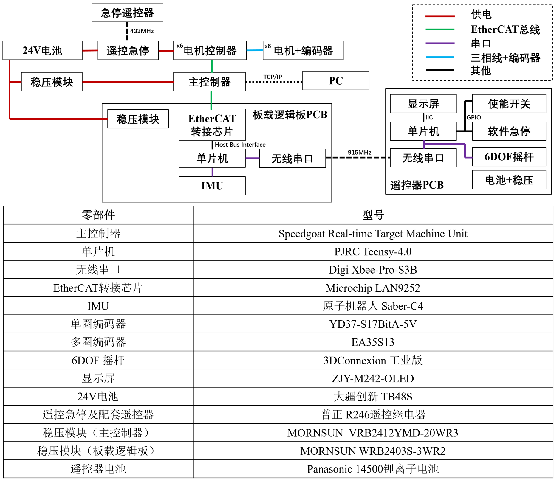
\includegraphics[width=0.9\linewidth]{figures/Sec3/sys.png}
  \caption{
  上:电气系统示意图。下:示意图中关键零部件具体型号。
  }
  \label{fig:sec3-sys}
   \vspace{6pt}
\end{figure}

供电方面,电池将直接通过稳压模块为SpeedGoat主控制器供电,以即使在使用遥控急停的情况下也不会丢失数据;板载逻辑板的稳压模块与上述供电并联;然后遥控急停开关通过分电板直接连接电机控制器,遥控急停受一个单独的遥控器控制,可以切断所有电机的电源。

\begin{figure}[h!]
  \centering
  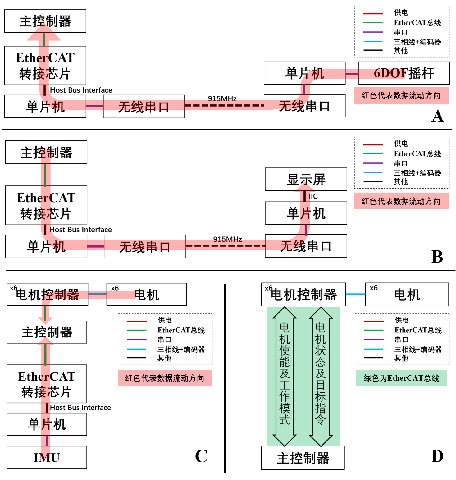
\includegraphics[width=0.9\linewidth]{figures/Sec3/comm.png}
  \caption{
  图A:运动控制指令由遥控器发送至主控制器处理。图B:机器人重要状态由主控制器发送至遥控器屏幕监看。图C:电机控制器、IMU反馈当前机器人状态给主控制器。图D:架设在电机控制器与主控制器间EtherCAT通讯网络上的两条虚拟通讯网络,分别是主控制器使能电机并决定电机工作状态,与主控制器发送电机与工作状态相应的运动指令。
  }
  \label{fig:sec3-comm}
   \vspace{6pt}
\end{figure}

通讯方面,最高层的通讯使用EtherCAT总线,使用菊花链的接线方式连接板载逻辑板、电机控制器和SpeedGoat主控制器。此外也可以使用TCP/IP与PC上位机的MATLAB Simulation进行通讯,实现程序下载、运行数据监看和参数调整等。板载逻辑板上的Teensy单片机会将EtherCAT总线中必要的数据,如电机的工作模式、电流等信息通过Xbee发送到遥控器以实现数据监看,遥控器也会回传运动指令。此外,遥控器可以远程静能所有电机,实现软件层面的另一种急停。IMU输出也是由该单片机将串口信号转换成EtherCAT信号。在这里,板载逻辑板内部的通讯构架是串口与Xbee提供的无线串口抽象。电机与电机控制器的通讯与控制是同时进行的:电机的转子位置信息通过编码器传输给电机控制器,而电机控制器直接传输驱动电流。

在EtherCAT通讯总线上,虚拟抽象出了以下两种数据链路:其一是用于决定电机使能静能、工作状态的底层控制数据链路;其二则是电机的转子位置、转子速度、转子加速度,和IMU的姿态、6轴加速度、6轴速度,作为系统的反馈提供给观测器,以获取状态变量。

\subsection{驱动模块}

驱动模块对于轮腿机器人而言至关重要,不但轮腿机器人的运动完全来自于驱动模块,而且驱动模块决定了机器人整体的性能。驱动模块包括电机本身、减速器、电机控制器和编码器等传感器。在上一章中,电机及其用途、机械性能已经被展示了,且准直驱电机包括了电机本身与减速器,因此下文所指的电机将包括减速器。在这里,更详细的电机的尺寸与电气参数如图\ref{fig:sec3-motors}所示。

\begin{figure}
  \centering
  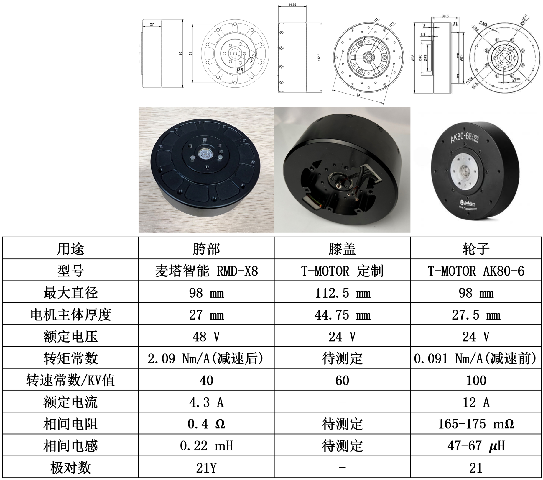
\includegraphics[width=0.85\linewidth]{figures/Sec3/motors.png}
  \caption{
  上图:电机尺寸。下图:尺寸及电气参数。
  }
  \label{fig:sec3-motors}
   \vspace{6pt}
\end{figure}

如上文所述,电机控制器通过编码器的位置反馈控制电机,且可以工作在包括位置模式、速度模式、电流模式等若干个模式。而在使用之前,需要但对每个电机进行三环调试。虽然轮腿工作在力控模式下时,无需调试速度和位置模式,但这些模式对初始化与实验调试必不可少。
准直驱的力控模式的实现原理是,根据电流和电动机的扭矩常数、减速比,计算出输出扭矩,也可以根据期望扭矩计算出目标电流。而扭矩常数往往有偏差或电机本身线性程度不好,需要对电机进行标定并选取工作范围内的数据,重新计算扭矩常数。
如引言所述,对于SpeedGoat中抽象的控制程序,电机的状态反馈必不可少,而电机控制器会根据编码器位置信息,计算出上述需求的反馈量。

\subsubsection{电机三环调试}
三环调试是指上一节所说的位置模式、速度模式和电流模式。其中电流模式是在输入和标定电机参数之后,通过伺服控制器内建的控制器实现电流环。在此基础上,通过PI控制器是实现速度环,而控制器的参数则是需要根据电机跟踪效果调节的。再在速度环的基础上,通过P控制器实现位置环,同样P参数也需要通过电机跟踪效果调节。调试过后这些参数保存在控制器中。

\subsubsection{电流-扭矩关系标定}
电机的扭矩在一定范围内与电流有很强的线性关系,虽然扭矩常数随电机转速会发生变化,但考虑到轮腿的工况,简化起见,仅标定静止状态下的电机扭矩常数。由于目前膝盖、胯部电机主要工作在位置模式,所以本毕设仅标定了轮子电机,但实际上电机的标定过程是相同的。如图\ref{fig:sec3-tauIplot}所示,标定的方式是,给定斜坡电流信号,然后通过力传感器读出已知距离处产生的力,便可根据力臂计算出扭矩。在获取原始的扭矩-电流信息后,选取实际工况所在范围,然后通过最小二乘的方式计算出斜率,从而计算出扭矩常数,如图\ref{fig:sec3-tauIplot}所示。

\begin{figure}
  \centering
  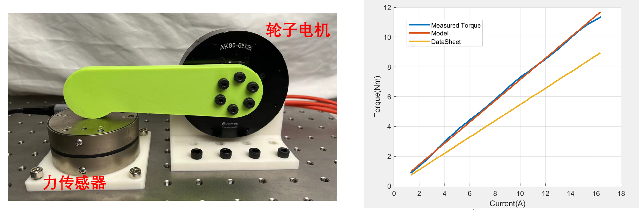
\includegraphics[width=0.85\linewidth]{figures/Sec3/tauIplot.png}
  \caption{
  左图:电机电流扭矩曲线测定实验平台。右图:电流扭矩实际曲线、根据最小二乘计算的曲线和厂商说明书给定的曲线。
  }
  \label{fig:sec3-tauIplot}
   \vspace{6pt}
\end{figure}

\subsubsection{电机控制器和编码器}
电机控制器和编码器的详细型号如图\ref{fig:sec3-escen}所示。电机控制器除了接受对应工作模式的指令、反馈电机的状态外,在进入这些模式之前,需要使能。与之相对应的,当电机驱动器静能之后,电机便不再输出扭矩。静能只需要将电机控制器的CMD WORD置为0,而出于安全考虑,使能过程较为复杂,以防止电机误使能发生意外。概括而言,电机驱动器会周期性发送STATUS WORD,主控制器需要连续若干次根据事先约定的计算方式根据STATUS WORD计算出正确的CMD WORD以使能电机,具体如图\ref{fig:sec3-motoren}所示。
使能后,电机驱动器通过OP MODE信息决定工作模式,会将与工作模式对应的指令作为目标状态,控制电机达到这些状态,而电机的工作状态,也就是上文提到的实际转子位置、速度、加速度、电流等等都以EtherCAT的通讯频率发送至主控制器。
关于编码器,值得注意的是,轮子编码器并需要绝对位置信息,而其他电机使用绝对位置编码器,具有断电后保存的功能,使得每次机器人初始化无需进行工作空间和电机行程的标定。但仍然必须进行工作空间和电机行程的标定,并作为配置文件记录在主控制器中。

\begin{figure}[h!]
  \centering
  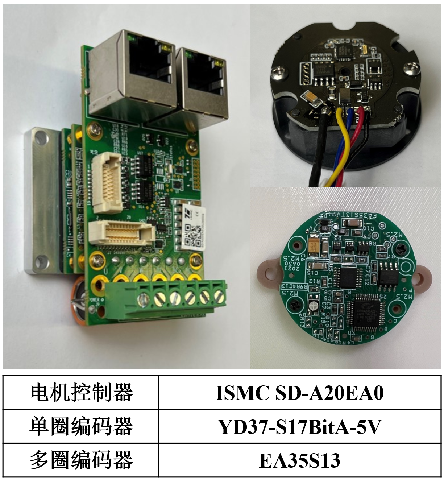
\includegraphics[width=0.6\linewidth]{figures/Sec3/escen.png}
  \caption{
  左图:电机控制器。右上图:单圈编码器,用与轮子电机。右下图:多圈编码器,用于膝盖、胯部的电机,需要外接电池,可以机器人关闭后保存位置信息,当机器人启动后,电池会自动充电;保存位置信息使得机器人免于每次上电时都需要校准膝盖和胯部的行程。
  }
  \label{fig:sec3-escen}
   \vspace{6pt}
\end{figure}

\begin{figure}
  \centering
  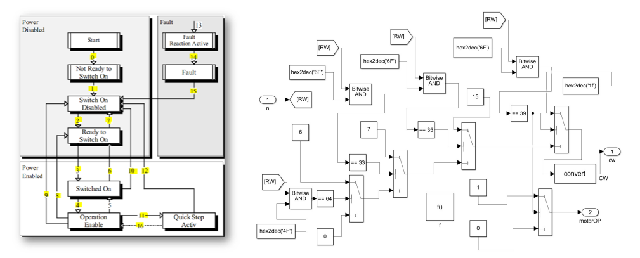
\includegraphics[width=0.85\linewidth]{figures/Sec3/motoren.png}
  \caption{
  左图:电机驱动器中关于电机使能方式的说明。右图:实际在Simulink中的使能程序截图。
  }
  \label{fig:sec3-motoren}
   \vspace{6pt}
\end{figure}

\subsection{SpeedGoat控制器}
SpeedGoat控制器是基于QNX操作系统的商业化实时工业控制器,其支持EtherCAT、CAN等通讯,使用MATLAB Simulink进行编程,相比于传统的基于Linux和ROS的PC作为控制器,具有敏捷开发、硬件实时、便于数据监看与记录、减少并行化程序错误的优点。本毕设采用的SpeedGoat控制器的如图\ref{fig:sec3-speedgoat}所示,其体积与功耗较小,但可实现EtherCAT总线1000Hz的通讯,且对EtherCAT通讯支持较好。使用MATLAB Simulink进行编程时,可以留出统一接口,方便将为MATLAB Simulink Simscapes仿真模型设计的控制器迁移到实物,或实现数字孪生功能。Simulink编程解决了并行化的大多数问题,如内存同时访问,资源上锁、调度等,且提供直观的数据监看和记录,并可以在MATLAB中进行快速处理。Simulink也可以调用MATLAB程序,并编译执行,以实现与编译型语言类似的执行速度;MATLAB则提供了丰富高效的线性代数、优化、学习、机器人运动控制等库,且编程简单快速。使用这种开发模式,可以实现一种类似于元编程(Meta-programming)的效果。

\begin{figure}
  \centering
  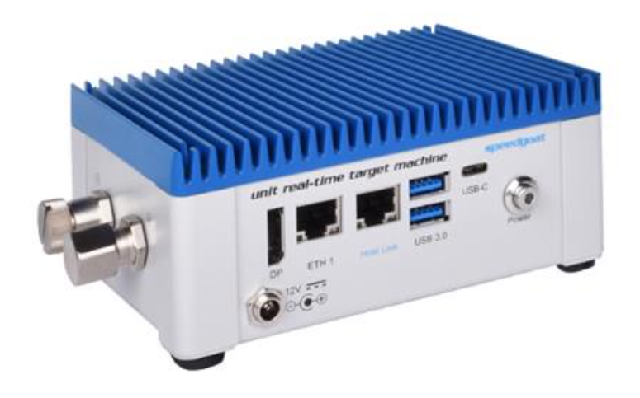
\includegraphics[width=0.6\linewidth]{figures/Sec3/speedgoat.png}
  \caption{
  Speedgoat Real Time Target Machine Unit示意图。
  }
  \label{fig:sec3-speedgoat}
   \vspace{6pt}
\end{figure}

\subsection{板载逻辑板等部件}
如引言所述,板载逻辑板包括了稳压模块,Teensy 4.0 单片机,EtherCAT转接芯片,IMU和Xbee。其具体如图\ref{fig:sec3-logicbd}所示。其中稳压模块负责供电,而Teensy单片机负责将数据从Xbee传入和传出EtherCAT总线,并将IMU数据转换至EtherCAT总线。
Teensy单片机支持开源Arduino社区的库,并可以使用与Arduino相同的方式编程,但其芯片采用ARM Cortex-M7内核,核心频率高达600MHz,且可以超频的超线程处理;其拥有丰富的外设和GPIO,并且CPU具有缓存及分支预测设计,并支持32位浮点数和DSP指令。其体积小巧,开发快速。
Xbee是Digi公司根据ZigBee协议设计的多功能无线串口。其延迟约为数十毫秒,体积小,功耗低,但连接稳定,调试方便,带宽大。Teensy单片机会从EtherCAT总线读取电机和IMU的状态,然后通过Xbee发送至遥控器及数据监看;而遥控器会给出运动指令,并兼具初始化电机使能和软件急停的功能,这些信息也都通过Teensy从Xbee读出后发送至EtherCAT总线,然后通过SpeedGoat主控制实现。Teensy单片机完全负责通讯转换的工作。

\begin{figure}
  \centering
  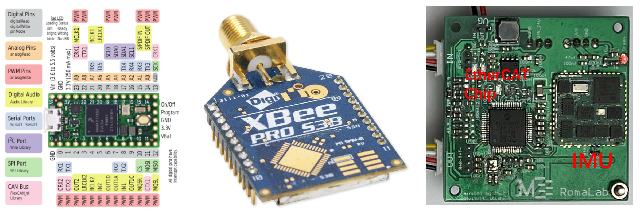
\includegraphics[width=0.85\linewidth]{figures/Sec3/logicbd.png}
  \caption{
  左图:Teensy单片机。中图:Xbee模块。右图:IMU及EtherCAT转接芯片。
  }
  \label{fig:sec3-logicbd}
   \vspace{6pt}
\end{figure}

\subsection{遥控及数据监看}

\begin{figure}[h!]
  \centering
  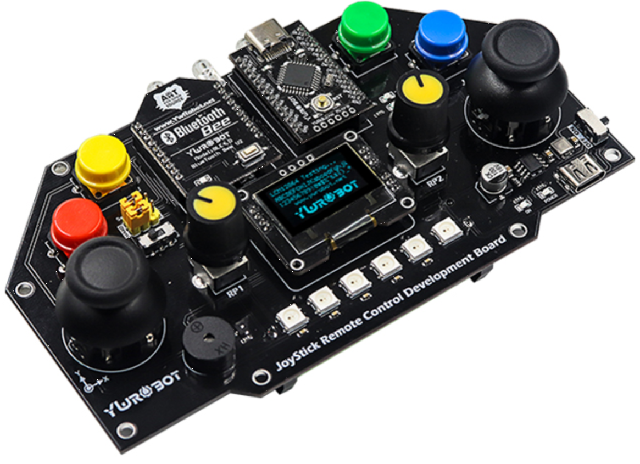
\includegraphics[width=0.75\linewidth]{figures/Sec3/rmctrl.png}
  \caption{
  遥控器示意图
  }
  \label{fig:sec3-rmctrl}
   \vspace{6pt}
\end{figure}

考虑到市面上成熟的RC遥控器多使用PPM或者Sbus通讯协议,并仅支持少数简单传感器信号回传,而轮腿机器人回传信息较为复杂。且这些遥控器虽然控制模型飞机,但其使用两个XY摇杆控制,仅能控制4自由度运动,操作并不直观。因此本毕设自主设计了遥控器,其系统图如图\ref{fig:sec3-rmctrl}。

其中3Dconnexion摇杆具有6个自由度,虽然轮腿仅能实现至多4个自由度的单独控制,但该摇杆非常直观,与运动指令一一对应,而无需考虑XY摇杆的映射问题。Xbee负则实现无线通讯,Teensy单片机则将机器人回传的信息通过串口读出,并通过OLED屏幕或RGB指示灯显示。而机器人的电机使能和静能,软件急停和上述运动控制指令也通过Xbee发送到机器人。

\subsection{本章小结}

本章介绍了电气系统。首先介绍了电气系统的整体框图,包括EtherCAT总线及挂载在总线上的各个设备,包括电机驱动器、主控制器和IMU,并逐一介绍他们。在介绍电机驱动器时,同时介绍了编码器、电机的三环调试和电流、扭矩曲线标定。在介绍IMU的部分,同时介绍了遥控通讯系统和遥控器的设计及数据监看。
\clearpage
% !Mode:: "TeX:UTF-8"
% !TEX program  = xelatex

% \section{一些样例}

% \subsection{表格}

% \begin{table}[htb]
% % h-here,t-top,b-bottom,优先级依次下降
%     \begin{center}
%     % 居中
%         \caption{表格的标题应该放在上方}\label{table}
%         \begin{tabular}{lc} % 三线表不能有竖线,l-left,c-center,r-right
%             \toprule
%             %三线表-top 线
%             Example & Result \\
%             \midrule
%             %三线表-middle 线
%             Example1          & 0.25 \\
%             Example2          & 0.36 \\
%             \bottomrule
%             %三线表-底线
%         \end{tabular}
%     \end{center}
% \end{table}

% \subsection{参考文献}

% 参考文献如是\cite{Nicholas1998Handbook}。

\section{建模与控制}

\subsection{引言}
机器人建模与控制是机器人研究中最重要的话题之一。机器人的建模既是研究者所关心的状态量与输入量之间的关系(例如输入关节电机角度,与输出末端位姿之间的关系),也可以是研究者所关心的量之间的关系(例如末端的速度,与关节速度的关系)。实际上,考虑到自然界的许多过程广泛设计动态系统,即其系统模型通常以常微分方程或偏微分方程所描述,实际上机器人建模也是状态量自身现在与过去的关系。而对于机器人而言,实际上所有刚体机器人建模归根结底都可以表达为描述了机器人全部的微分方程,这里强调刚体是因为刚体机器人中状态数目是有限的,而软体机器人的状态甚至不是可数(countable)的,而从上述方程中,通过选取部分、抽象封装的方式,便可以获得需要研究的建模内容。具体而言,读者可能会反驳如何从刚体机器人的动力学模型中获得正向或者逆向的位置运动学,而笔者的论点是:将电机能够提供位置模式、速度模式这样具体的想法便已然是一种抽象与封装。对于电动机而言,其无法静态地、开环地、稳定地提供速度或者位置地输出,实际上其运动地一切根源均来自牛顿第三定律。因而,其输出扭矩到输入电流之间便有一种理想的映射,并以电动机转矩常数冠名。读者可能会继续反驳,在电动机内部,难道就是这样理想的映射?笔者则继续解释称,理想电动机内部如是,但实际电动机存在转子惯量和线圈电感,因而并不能认为是给定电流便理解输出相应扭矩的模型,自然会有同样的动态过程。而进一步的,电动机也并不理想,因而上述电流到扭矩之间的映射也不是持续可靠,甚至在其工作范围内也不成立。因此,考虑到误差的可接受度,笔者也对其进行了一定的简化。具体而言电动机的转子和线圈对其输出扭矩的影响,分别以机械时间常数与电气时间常数称呼,来自于其动力学方程,一个一阶常微分方程中的时间常数。考虑到时间常数甚小,因此对机器人的影响较小,因而将之忽略,从而简化机器人动力学模型。如果归根结底地将电机的更上一级的电机控制器内部的动态过程也考虑进去,整个系统会变为混合系统,且更为复杂——因为在电机控制器中,不仅存在连续的动态系统,也存在离散的动态系统,即使是用于处理的逻辑芯片与存储数据的内存,其本质上与人类在发明他们时制造的三极管和电容无二异,芯片的设计也需要考虑流水线、寄存器的读取速度与时钟周期,并伴随着随机性的电压与校验错误的影响。因此,如果这些内容不加以抽象,整个动力学将会过于复杂。但是,抽象的程度并无确定性的答案,例如电机可抽象为电流环,也可抽象为速度环,还可抽象为位置环,这些都将取决于具体的情况所定。当然,对于抽象过的内容,一般也会有其性能表征,例如电机的机械时间常数与电气时间常数便是其性能表征的体现;而对于电机控制器和处理器,其能够运行的频率和延迟,也同样是性能表征的一部分。我们也可以用以这测试驱动开发(TDD,Test driven development)的方式理解,之所以要解开位置和速度的封装,有的时候时是因为单纯的位置或者速度控制隐藏了太多的内容,无法达到预期的表现,或者是现在的技术已经足以面对更加复杂的系统,对更加复杂的系统进行建模,则对其了解更多,控制效果更好。另一方面,电动机、电机控制器也不可能根据机器人科学家的想法进行随心所欲的定制,因此更多时候需要将他们假设成一个黑箱子(Oracle),面向可以获得的信息建模。这时候就有通过控制位置或者速度的方式实现力控了,读者不妨想象如下的过程:对于理想的机器人电机和控制器而言,如果规定机械臂需要执行的运动轨迹,则可以通过动力学方程反推出电机的扭矩;但如果使用理想的电机和控制器用位置逆解的方式跟踪,则此时检查电机的扭矩,便毫无疑问地会发现二者一致。在这里,笔者愿称之为孪生或者对偶,其实际上是同一件事情的两面。因此回到一开始读者的提问,便是如何从动力学模型中提取出运动学模型?在这里终于可以给出解答:利用动力学模型,反算出研究者关心的变量分别与动力学模型中所有变量的关系,然后进行化简即可。笔者在这里需要提及广义的方程组求解:对于线性方程组,朴素的解法是根据矩阵本身的特性求解,而或者是使用广义逆等方式求解,但其都可以划归为寻求满足方程约束的解与优化变量之间距离。根据距离函数(范数)的定义不同,如果是欧几里得范数,则可以被认为是一种二次规划(QP)问题。在这一段落的尾声,笔者必须指出:可以从动力学模型中获取运动学模型并不代表我们将这么做,实际上更多时候或许是不可能的,实际上本章剩余的部分也将遵循一种位置运动学-速度位置学-动力学的范式。这里想表达的是,运动学模型与动力学模型之间是并不割裂的,而是一种推广的关联关系,或者可以成为动力学模型“蕴含”(Entail)了运动学模型。

回到具体的轮腿机器人上,其一般被简化为小车-倒立摆(Cart-Pole)模型,是一种典型的欠驱动机器人,因此即使是简单的静态平衡也涉及相对多的控制算法。机器人在CAD软件设计之后,可以获得准确的尺寸和粗略的质量、质心位置和转动惯量参数,而由于仿真的自定特性,CAD模型可以直接用于构建仿真模型。但是实物原型机出于各种原因(部分零部件没有质量、质心数据),仍然需要进行单独的参数辨识。一般而言,参数辨识可以离线完成,也可以在线使用观测器实现。对于实现简单的平衡控制,通过离线测定重心位置的方式就有相对不错的效果。在线使用观测器则涉及了非线性的系统辨识,一般采用扩展卡尔曼滤波实现(EKF)。仿真模型可以认为是实物原型机的数字孪生。
在拥有必要的参数后,可以通过对机器人建模的方式研究其系统,一般而言,机器人拥有运动学和动力学模型,而控制器则通过这些模型和实际情况去设计。当机器人需要实现变高度时,由于胯部和膝盖电机都工作在位置模式,所以一般是使用位置运动学模型进行工作空间到关节空间的转换,然后使用位置模式去控制;而但机器人需要实现简单的PID平衡时,则需要根据机器人实现测定的重心位置,或者每个杆件的重心位置通过机器人构型计算出来的结果,去跟踪重心与竖直线的偏差,以实现控制;如果是使用LQR进行空间的轨迹跟踪,则需要根据动力学模型线性化为状态空间方程,并选取选哟控制的状态量,然后根据Q与R惩罚矩阵设计对应的状态变量增益K。其中涉及到的质心位置,可以通过实现测定和根据构型计算,也可以通过EKF进行观测,在线调整,例如在机器人被加载负载时,则只能通过上述在线调整方法。

\subsection{建模}
一般而言,运动学包括位置运动学正逆解和微分/速度运动学\cite{corke2011robotics}\cite{lynch2017modern}(雅可比运动学)。位置运动学正解是:给定驱动器的各关节角度,计算末端或指定刚体的位姿(pose),这在计算雅可比矩阵和动力学时有重要作用。
速度运动学,或雅可比运动学,是关节空间的速度和末端或指定刚体速度的映射关系,且是双射。雅可比矩阵可以运用在微分逆运动学控制中;由于空间力和速度的对偶关系,根据虚功原理,可以得出雅可比矩阵的转置同样是相同末端或指定刚体受到的合外力到关节空间扭矩的映射,称之为力雅可比矩阵。
对于任何机器人,欧拉-拉格朗日法都可以用于分析动力学,从而建立状态方程。但是这种方法对于符号计算和技巧要求较高,并不适合一些基于动力学的控制方法,因此对于固定基座的串联机器人,一般采用递归牛顿欧拉法,虽然这并不适用于轮腿机器人,但是可以首先假设轮子与地面关系,然后使用IMU的读书带入线性方程,从而解算出机器人扭矩和运动状态的关系。
基于动力学控制的优点显而易见:力是运动改变的原因,而电机无法在外界负载变换的情况下,对位置和速度进行高频的良好跟踪。电机负载越大,上述跟踪越差。而电机力控则可以实现高频跟踪,并且性能与负载无关。速度和位置的性能差的原因,来自于电机内部的控制器是无法接受外界信息,尤其是前馈信息的,因此很难在任何负载及负载变化下达到最优。而动力学控制正是根据需要跟踪的轨迹和机器人动力学模型反算出电机的前馈力矩,使得电机的反馈力矩是线性的,从而可以达到一致的较好效果。

\subsubsection{运动学模型}

本子节中,运动学模型既包括机器人本身部件之间的运动学模型,也包括机器人作为移动机器人的运动学模型。

关于机器人杆件之间的运动学模型,为了简化模型,目前仅对轮腿机器人的建立简单的矢状面(如图\ref{fig:sec2-3lim})运动学模型,考虑到轮子与地面并不固连且持续旋转,且认为机器人构型不会经常改变,因此选取z轴与小腿方向重合的坐标系B,根据膝关节和胯关节电机的角度以及对应杆件质量、长度,可以计算出质心位置和IMU位置,从而计算出IMU测量的俯仰角与实际上质心与铅垂线的偏差角度,从而利用此角度设计PID或LQR控制器。如图\ref{fig:sec4-frame}所示:

\begin{figure}
  \centering
  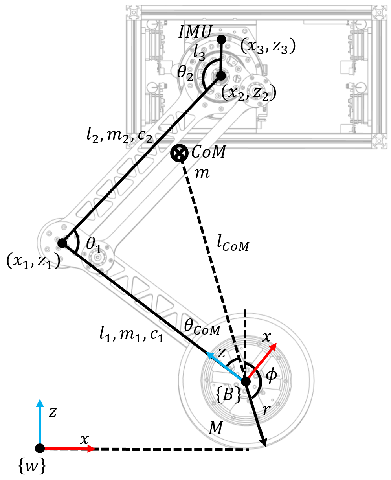
\includegraphics[width=0.5\linewidth]{figures/Sec4/frame.png}
  \caption{
  矢状面建模及相关物理量符号定义示意图。
  }
  \label{fig:sec4-frame}
   \vspace{6pt}
\end{figure}

其中轮腿变高度与电机角度的关系和上述角度偏差关系如下:
$\{w\}$为世界系, 而$\{B\}$是中心和轮子中心重合,但$z$方向总是指向膝关节的座标系。$\phi$轮子自从初始位置开始旋转过的角度,因而$x_B = \phi r,\ y_B = r$.小腿和大腿的质量、长度和质心位置分别是$(l_1,m_1,c_1),\ (l_2,m_2,c_2)$,这些数据都可以从CAD模型中获得。$\theta_1,\ \theta_2$则由膝关节和跨关节的电机决定,且如果机器人完全直立站起,$\theta_1 = \theta_2 = \pi$.机器人躯干的质心被认为是与胯关节的中心重合,而IMU安装在距离中心$l_3$的位置。于是我们可以计算在$\{B\}$系下的质心位置:
\begin{equation}
\begin{bmatrix}
    x_{CoM} \\
    z_{CoM}
\end{bmatrix}
=
\frac{
\sum_i^{} m_i
\begin{bmatrix}
    x_{c_i} \\
    z_{c_i}
\end{bmatrix}
}{\sum_i^{} m_i}
\label{eq:com_calc}
\end{equation}

类似的,在$\{B\}$系下的每个点的坐标可以用如下的公式计算出来:
\begin{equation}
\begin{bmatrix}
    x_{c_1} \\
    z_{c_1}
\end{bmatrix}
=
\begin{bmatrix}
    0 \\
    c_1
\end{bmatrix}
    \label{eq:kine_c1}
\end{equation}

\begin{equation}
    \begin{bmatrix}
        x_{c_2} \\
        z_{c_2}
    \end{bmatrix}
    =
    \begin{bmatrix}
        c_2 sin\theta_1 \\
        l_1 - c_2 cos\theta_1
    \end{bmatrix}
    \label{eq:kine_c2}
\end{equation}

\begin{equation}
    \begin{bmatrix}
        x_{c_3} \\
        z_{c_3}
    \end{bmatrix}
    =
    \begin{bmatrix}
        l_2 sin\theta_1 \\
        l_1 - c_2 cos\theta_1
    \end{bmatrix}
    \label{eq:kine_c3}
\end{equation}

从根据公式\ref{eq:com_calc},公式\ref{eq:kine_c1},公式\ref{eq:kine_c2} 和公式\ref{eq:kine_c3}中,我们可以计算${B}$系下的等效质心位置。而要计算质心与竖直线之间的夹角,我们需要结合质心位置与IMU测量数据。IMU在${B}$系下的位置是:

\begin{equation}
    \begin{bmatrix}
        x_3 \\
        z_3
    \end{bmatrix}
    =
    \begin{bmatrix}
        l_2 sin\theta_1 - l_3 sin(\theta_1 - \theta_2) \\
        l_1 - l_2 cos\theta_1 + l_3 cos(\theta_1 - \theta_2)
    \end{bmatrix}
    \label{eq:kine_3}
\end{equation}

那么IMU和质心之间的夹角就是

\begin{equation}
    \theta_{CoM} = atan2(z_3 - z_{CoM}, x_3-x_{CoM})
    \label{eq:theta_com}
\end{equation}

由于IMU直接测量了其与竖直线之间的夹角$\theta_{IMU}$,所以质心与竖直线之间的夹角是:

\begin{equation}
    \theta = \theta_{IMU} + \theta_{CoM}
    \label{eq:theta_calc}
\end{equation}

\begin{figure}[h!]
  \centering
  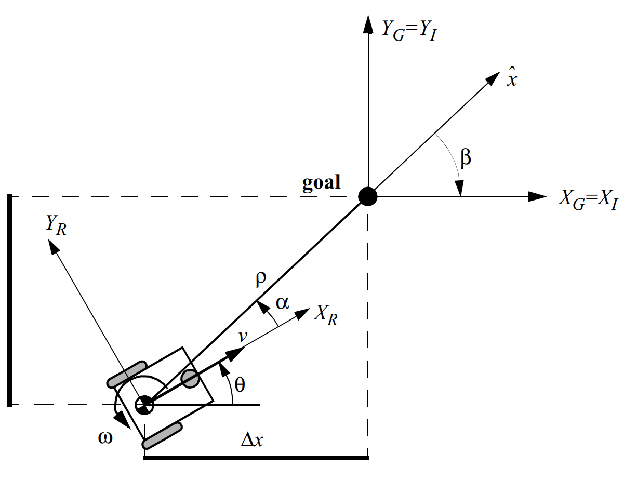
\includegraphics[width=0.6\linewidth]{figures/Sec4/kingoal.png}
  \caption{
  移动机器人动力学示意图\cite{siegwart2011introduction}。
  }
  \label{fig:sec4-kingoal}
   \vspace{6pt}
\end{figure}

而考虑移动机器人动力学时,本轮腿机器人由两个差速转向的轮子控制运动,具体如图\ref{fig:sec4-kingoal}所示。取$[x,y,\theta]^T$为机器人的状态变量,则机器人的状态与其线速度、角速度的关系如公式\ref{eq:stalinang}所示。

\begin{equation}
    \begin{bmatrix}
        \dot{x} \\ \dot{y} \\ \dot{\theta}
    \end{bmatrix} = 
    \begin{bmatrix}
        cos \theta & 0 \\ sin \theta & 0 \\ 0 & 1
    \end{bmatrix}
    \begin{bmatrix}
        v \\ \omega
    \end{bmatrix}
    \label{eq:stalinang}
\end{equation}

考虑到后文中提到机器人需要进行轨迹跟踪,因此在给定如图\ref{fig:sec4-kingoal}中的目标点后,我们需要计算其中的参数$\alpha$、$\beta$和$\rho$。在这里将采用极坐标转换如公式\ref{eq:cat2rho}所述,变换为如公式所述的形式,于是可以得到机器人与目标点之间的关系,而利用这个关系可以作为反馈控制,以达到给定的目标点。
\begin{equation}
    \begin{aligned}
      \rho & = \sqrt{\Delta x^2 + \Delta y^2} \\
      \alpha & = -\theta + atan2(\Delta y, \Delta x) \\
      \beta & = -\theta -\alpha 
    \end{aligned}
    \label{eq:cat2rho}
\end{equation}

\begin{equation}
    \begin{bmatrix}
        \dot{\rho} \\ \dot{\alpha} \\ \dot{\beta}
    \end{bmatrix} = 
    \begin{bmatrix}
        -cos\alpha & 0 \\ \frac{sin \alpha}{\rho} & -1 \\ -\frac{sin\alpha}{\rho} & 0
    \end{bmatrix}
    \begin{bmatrix}
        v \\ \omega
    \end{bmatrix}
\end{equation}

而对于机器人的速度$[v,\omega]^T$与机器人轮速之间的关系,假设机器人轮间距为$2d$,则不难推出其关系如公式所示。
\begin{equation}
    \begin{bmatrix}
        v \\ \omega
    \end{bmatrix} = 
    \begin{bmatrix}
        \frac{1}{2} & \frac{1}{2} \\ \frac{1}{d} & -\frac{1}{d}
    \end{bmatrix}
    \begin{bmatrix}
        v_1 \\ v_2
    \end{bmatrix}
    \label{eq:naveq}
\end{equation}

\subsubsection{动力学模型}
正如引言中所述,力是运动改变的原因。对于固定底座的机械臂而言,即使不考量动力学模型,依然可以通过位置控制或者微分逆运动学进行速度控制来实现轨迹跟踪。虽然在PID平衡中,动力学也可以不考虑,但是其进行矢状面轨迹跟踪是依靠对轮子编码器的加权和饱和作为偏差输入到控制器中,这种控制方式虽然能实现效果,但需要仔细调整权重和饱和;而一般而言,对于轮腿机器人来说,如果有动力学模型则可以获知整个系统的向量场,从而使用LQR的方式收敛到任意的向量场中可控的一点。
考虑到轮腿机器人的膝关节和胯关节工作在位置模式下,因此并不考虑腿部的动力学,而轮腿的轮子转动惯量先对于系统其他部分对动力学的影响较小,因此可以忽略,则轮腿可以简化成小车-倒立摆模型。这里倒立摆并不视为一个质点,因此需要计算转动惯量。其中一种方式是利用CAD模型给出的粗略的转动惯量矩阵,在坐标变换后相加,然后计算绕轮子中心轴的转动惯量。另一种方式是将每个杆件视为质点,然后利用平行轴定理计算转动惯量之后相加。由于整体的质心位置也需要使用机器人构型计算,因此在实际控制中,采用的是后一种方式。

为了更简便的控制,我们对膝关节和胯关节电机采取静力学假设。如公式\ref{eq:com_calc}所示,质心在${B}$系下的位置,和整个机器人在其中的转动惯量都是与膝盖和胯部电机有关的函数。为了进一步简化,我们假设所有杆件都是质点,这样可以根据每个杆件的质心计算公式\ref{eq:kine_c1},公式\ref{eq:kine_c2}和公式\ref{eq:kine_c3},所有杆件(除了轮子)的转动惯量式:
\begin{equation}
    I = 2m_1 (x_{c_1}^2+z_{c_1}^2) + 2m_2 (x_{c_1}^2+z_{c_1}^2) + m_3 (x_{c_1}^2+z_{c_1}^2)
    \label{eq:inertia}
\end{equation}

\begin{figure}
  \centering
  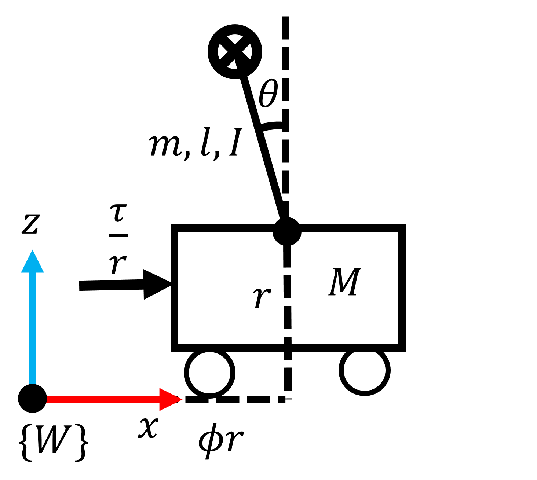
\includegraphics[width=0.4\linewidth]{figures/Sec4/2dsimple.png}
  \caption{
  矢状面动力学模型符号定义示意及小车-倒立摆模型建图。
  }
  \label{fig:sec4-2dsimple}
   \vspace{6pt}
\end{figure}

由于轮子的转动惯量较小,相对于整个机器人,其影响机器人的动力学较少,因此机器人可以简化成一个小车-倒立摆模型。我们定义$f = \frac{\tau}{r}$以及$x = \phi r$,这样我们使用欧拉-拉格朗日公式就可以计算出动力学模型。在这里,我们首先考虑矢状面的动力学模型,然后考虑空间中的动力学模型。其中机器人的矢状面定义如图\ref{fig:sec2-3lim},而其简图如xxx所示。除了欧拉-拉格朗日公式,还可以使用另外两种分析方式,这里也将详细展开。欧拉-拉个朗日法聚焦于能量视角,其中系统的广义位置、广义速度分别为$q$,$\dot{q}$,对应的广义力为$   \tau$,针对广义速度可计算出系统的整体的动能$T$与势能$V$,并定义$L=T-V$则可以用公式\ref{eq:eu-la}求出广义力:

\begin{equation}
    \tau = \frac{\partial L}{\partial \dot{q}} - \frac{\partial L}{\partial q}
    \label{eq:eu-la}
\end{equation}

对于本轮腿机器人,上述动能为小车部分与倒立摆的动能之和:

\begin{equation}
    T=\frac{1}{2}(M+m)\dot{x}^2 + m\dot{x} \dot{\theta} l cos \theta + \frac{1}{2} m l^2 \dot{\theta}^2
    \label{eq:la-T}
\end{equation}

而势能则只与倒立摆的角度,相应的质心高度,有关:

\begin{equation}
    U=-mglcos \theta
    \label{eq:la-V}
\end{equation}

通过式\ref{eq:eu-la},式\ref{eq:la-T},式\ref{eq:la-V},可以计算系统的动力学方程如下:

\begin{equation}
    (M+m)\ddot{x} - ml\ddot{\theta}cos\theta -ml\dot{\theta}^2 sin\theta = f
    \label{eq:motion1}
\end{equation}

\begin{equation}
    ml^2\ddot{\theta} + mgl sin\theta = ml\ddot{x}cos\theta
    \label{eq:motion2}
\end{equation}

\begin{figure}
  \centering
  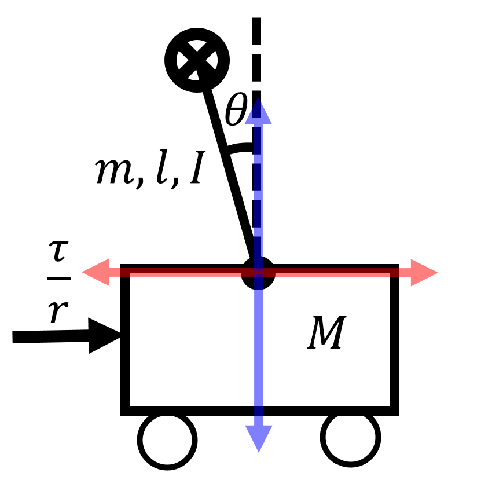
\includegraphics[width=0.4\linewidth]{figures/Sec4/2d2.png}
  \caption{
  矢状面受力分析图(F.B.D.)符号定义。
  }
  \label{fig:sec4-2d2}
   \vspace{6pt}
\end{figure}

接下来讨论另一种简单的基于分析的方法,以及它的牛顿-欧拉法的变种,最后使用这种方法推广到三位空间中的线性倒立摆模型。首先我们考虑朴素的受力分析方法,具体来说,首先分析每个被隔离的杆件。具体各种力的定义如图\ref{fig:sec4-2d2}所示,关于小车的受力如公式\ref{eq:cart-f}所示。
\begin{equation}
    M\ddot{x} = F - N
    \label{eq:cart-f}
\end{equation}
而关于铰链处的力$N$的表的是则如公式\ref{eq:cart-n}所示。
\begin{equation}
    N = m\ddot{x} + ml\ddot{\theta}cos \theta - ml\dot{\theta}sin \theta
    \label{eq:cart-n}
\end{equation}
接着沿着倒立摆方向的受力如公式\ref{eq:cpf}所示。
\begin{equation}
    Psin\theta N cos\theta - mgsin \theta = ml\ddot{\theta} + m\ddot{x} cos\theta
    \label{eq:cpf}
\end{equation}
通过转矩关系(公式\ref{eq:pnrel})消去$P$和$N$以获得最终的结果。

\begin{equation}
    -Plsin\theta - Nlcos\theta = I\ddot{\theta}
    \label{eq:pnrel}
\end{equation}

最终得到与公式\ref{eq:motion1}和公式\ref{eq:motion2}相同的结果。

在这里,我们可以总结出牛顿欧拉法的具体使用方式:首先确定所有杆件,并据此定义状态变量。每个刚体具有6个自由度,定义杆件数$\times$6的状态变量之后,首先寻找杆件自身的约束,如杆件固定在地面上,或杆件须沿指定轴旋转(相应的便是5维的约束力),然后寻找相关杆件之间的约束,大多数机器人关节都可以用极简易的方式定义,一些相对复杂的例如圆柱沿斜面无滑动的滚动也可以首先找到可能的运动空间,然后寻找该运动的对偶空间,其基便是约束力。接下来,针对每个杆件,将与之相关的力,包括电机的扭矩、约束力、重力和约束力。值得注意的是,惯性力、科氏力(Coriolis Force)和陀螺力(Centrifugal Force)并不考虑在内,这是因为牛顿欧拉方程\cite{featherstone2014rigid}(如公式\ref{eq:newtoneul})已经将他们考虑在内了。

\begin{equation}
    \mathcal{F} = \mathcal{I}\mathcal{A} + \mathcal{V}\times^* \mathcal{I} \mathcal{A} + \mathcal{J}^T\mathcal{F}_{ext}
    \label{eq:newtoneul}
\end{equation}

在上述公式中,所有杆件必须换算在同一坐标系下。其中$\mathcal{I}$是空间转动惯量,$\mathcal{V}$是空间速度,$\mathcal{A}$是空间加速度,$\mathcal{J}$是接触力的雅可比矩阵,$\mathcal{F}$是空间力,$\times^*$是定义在空间速度上的叉乘,是一个确定的线性变换,甚至可以认为是同构,具体而言就是将空间速度这一6维向量转换成了一个6$\times$6的矩阵形式。上述讨论产生的方程组在有时出于“未知数过多,方程太少”的原因会有多解,例如轮腿机器人这一欠驱动系统,轮子与地面之间的接触无法检测,因此相应的甚至无法建立相应的方程。此时考虑轮腿上的传感器IMU,可以根据轮腿的其他关节的运动状态计算出轮子与地面之间的接触模型。

\begin{figure}
  \centering
  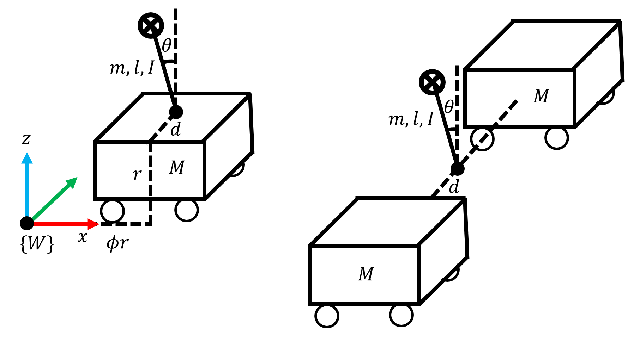
\includegraphics[width=0.45\linewidth]{figures/Sec4/3dsimple.png}
  \caption{
  空间的动力学模型符号定义示意及小车-倒立摆模型建图。其中左图是是空间中的小车-倒立摆模型的示意图,右图则是进一步简化后,将左右轮分别视为两个小车,然后研究其上倒立摆的模型。
  }
  \label{fig:sec4-3dsimple}
   \vspace{6pt}
\end{figure}

对上述过程进行简化,接下来将推导空间的动力学模型。在这里依然采用小车-倒立摆模型,但是小车可以在二维平面上运动,如图\ref{fig:sec4-3dsimple}所示。其中考虑到轮子只能提供单自由度的转动,因此将其使用非完整约束如等式\ref{eq:3d-noh}所示。更加直观的说,每个轮子的速度只能与当前轮子的方向相同。

\begin{equation}
    \frac{\dot{y}}{\dot{x}} = tan \theta
    \label{eq:3d-noh}
\end{equation}

为简化计算,将两个轮子中间与倒立摆铰链连接的部分视为没有质量的物体,于是其位姿便于两个轮子的位置有如同等式\ref{eq:mid-pos}的关系。

\begin{equation}
    \begin{bmatrix}
        x \\
        y \\
        \theta 
    \end{bmatrix} = 
    \begin{bmatrix}
        \frac{x_1+x_2}{2} \\
        \frac{y_1+y_2}{2} \\
        atan2(y_2-y_1, x_2-x_1)
    \end{bmatrix}
    \label{eq:mid-pos}
\end{equation}

在此基础上,考虑二维小车-倒立摆模型,但是其中需要加上小车自转产生的角速度产生的陀螺力,使得公式\ref{eq:motion1}需要被修改为公式\ref{eq:motion3}。

\begin{equation}
    (M+m)\ddot{x} - ml\ddot{\theta}cos\theta - ml\dot{\theta}^2 sin\theta + \omega^2 lsin\theta cos\theta = f
    \label{eq:motion3}
\end{equation}

然后使用公式\ref{eq:mid-pos}反解出左右轮与中心点的关系并带入公式\ref{eq:motion1}和\ref{eq:motion3}中,即可得到机器人的三维空间中的动力学方程。

\subsubsection{状态空间方程}
一般而言,根据状态变量的选取,通过对动力学模型进行变换即可得到状态空间方程。这里令$u = f$,并取$[x,\dot{x}, \theta, \dot{\theta}]^T$作为状态变量,我们可以根据上述动力学模型(公式\ref{eq:motion1}和\ref{eq:motion2})获得矢状面的连续时间的状态空间方程:
\begin{equation}
    \begin{bmatrix}
        \dot{x} \\
        \ddot{x} \\
        \dot{\theta} \\
        \ddot{\theta}
    \end{bmatrix}
    =
    \begin{bmatrix}
        0 & 1 & 0 & 0 \\
        0 & 0 & \frac{m^2gl^2}{I(M+m)+MmI^2} & 0 \\
        0 & 0 & 0 & 1 \\
        0 & 0 & \frac{mgl(M+m)}{I(M+m)+MmI^2} & 0
    \end{bmatrix}
    \begin{bmatrix}
        x \\
        \dot{x} \\
        \theta \\
        \dot{\theta}
    \end{bmatrix}
    +
    \begin{bmatrix}
        0 \\
        \frac{I+ml^2}{I(M+m)+Mml^2} \\
        0 \\
        \frac{ml}{I(M+m)+Mml^2}
    \end{bmatrix}
    u
\end{equation}

如之前的章节所述,所有的状态变量,都可以通过IMU和轮子编码器读到。考虑到主控制器的选型与编程方式,这里需要对连续时间系统进行离散化。对于如公式\ref{eq:cl-sys}所示的连续时间系统,其离散化后如公式\ref{eq:dl-sys}所示。

\begin{equation}
    \begin{aligned}
    \dot{x} & = Ax + Bu \\
    y & = Cx + du
    \end{aligned}
    \label{eq:cl-sys}
\end{equation}

\begin{equation}
    \begin{aligned}
    x_{k+1} & = A_d x_k + B_d u_k \\
    y_k & = C_d x_k + D_d u_k \\ 
    A_d & = A + I \Delta t A \\
    B_d & = B \Delta t \\
    C_d & = C \\
    D_d & = D 
    \end{aligned}
    \label{eq:dl-sys}
\end{equation}

\subsection{控制}

\subsubsection{PID轨迹跟踪}
PID是一种广泛在工业界采用的控制其。其中缩写PID所代表的意思分别是比例、积分与微分。其具体控制原理的示意图如图\ref{fig:sec4-pidgram}所示,反馈量会与目标值进差值,然后对插值乘以一个比例作为控制量,同时对差值进行微分,然后在乘以一个比例叠加到刚刚的控制量上,最后对差值进行积分,乘以一个比例后在叠加至刚刚的控制量上,便成为了PID控制器。值得注意的是,其中的微分参数或者积分参数可以为0.

\begin{figure}[h!]
  \centering
  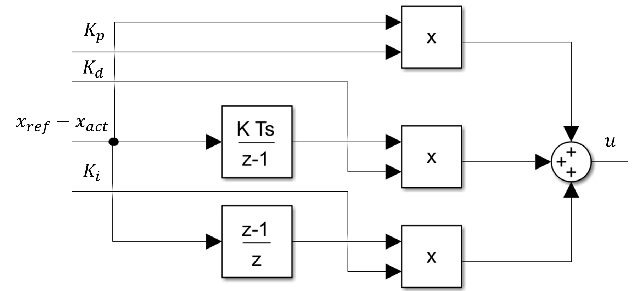
\includegraphics[width=0.75\linewidth]{figures/Sec4/pidgram.png}
  \caption{
  PID示意图
  }
  \label{fig:sec4-pidgram}
   \vspace{6pt}
\end{figure}

如前文所述,已知质心与竖直线夹角之后,可以建立PID控制器。但如果仅仅将期望位置加作为偏差,则控制器仅能保证机器人会位置在质心竖直向上的状态,但若质心测量稍有偏差,机器人就会维持一个恒定的加速度以维持平衡状态,而这显然是笔者所不希望看到的。此外,矢状面的轨迹跟踪的实现也与机器人在世界坐标系下的位置,也就是轮子编码器的具体角度息息相关,因此将轮子编码器当前值与目标值(目标位置)作为误差输入量之一输入PID控制器以实现矢状面的轨迹跟踪,如图\ref{fig:sec4-2dpid}所示。值得注意的是,考虑到机器人在失稳或者实验调试时轮子编码器可能会因为失败的平衡而记录错误的值,因此这里并不使用编码器上电值,而是平衡时且IMU读取线速度值极小时认为当前位置为原点。具体回到PID控制器,考虑到倾斜角度与机器人加速度相关,且当机器人质心接近于平衡状态时有$sin x \dot{=} x$,此时加速度实际上与倾斜角度成正比。因为可以使用此加速度控制机器人前进速度,而使用机器人前进速度控制机器人位置,因此可以将机器人的位置偏差作为输入量(系统观测量的偏差),将机器人的额外的倾斜角度作为输出控制量,叠加到上述PID控制器的角度偏差中。

\begin{figure}[h!]
  \centering
  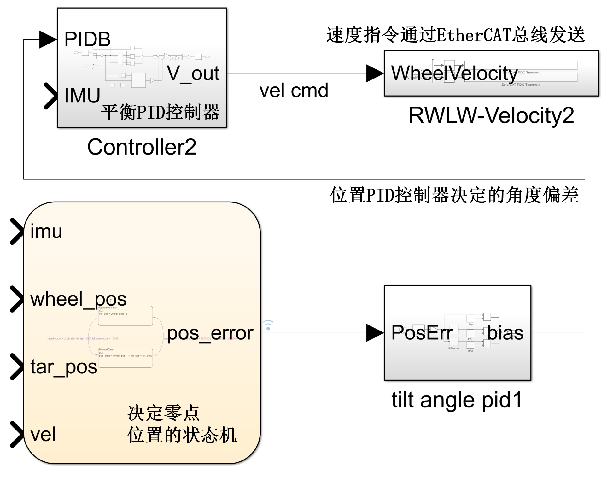
\includegraphics[width=0.75\linewidth]{figures/Sec4/2dpid.png}
  \caption{
  实际机器人矢状面PID控制器的示意图。
  }
  \label{fig:sec4-2dpid}
   \vspace{6pt}
\end{figure}

而转向则有差速转向开环实现,如图\ref{fig:sec4-3dpid}所示。当机器人接近平衡状态时,通过机器人角速度计算出每个轮子的速度差,从而叠加到轮子的指令速度上,再发送出去。当机器人不接近平衡状态时,此时机器人角速度会在质心产生陀螺力,从而影响机器人平衡状态,因此设有阈值,当机器人在平衡角度阈值内,才会执行转向指令。

\begin{figure}
  \centering
  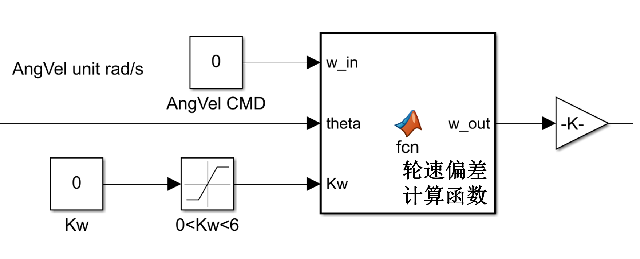
\includegraphics[width=0.8\linewidth]{figures/Sec4/3dpid.png}
  \caption{
  实际机器人3维轨迹追踪的差速转向控制器的示意图。其中输入量$Kw$是一个用于判定机器人倾角阈值的参数。
  }
  \label{fig:sec4-3dpid}
   \vspace{6pt}
\end{figure}

\subsubsection{LQR轨迹跟踪}
如前文所述,力是改变物体运动的原因。物体的运动可以通过物理定理,转化成微分方程,以方便研究。而已知物体运动的微分方程,也就知道可以在何种范围内修改物体的运动状态,以及以何种方式修改物体的运动状态。换句话说,在物体运动的状态空间中,控制是给出从当前状态到目标状态的路径(从路径可能随时间变化),将当前的全状态映射到可以控制的量上的函数,称之为控制率,如公式\ref{eq:ctrl_law}所示。
\begin{equation}
    u_{ctrl} = f(x_{state})
    \label{eq:ctrl_law}
\end{equation}
构建力与运动状态之间的关系并不是唯一可以用于控制的微分方程,但对于轮腿机器人这样欠驱动(underactuated)但可控(controllable)的系统,即使可以不使用力作为控制量,但使用力是最为简单与直观的。为简化控制,在得到状态空间方程如公式\ref{eq:dl-sys}所示后,便可以对可控的系统构建线性控制器。线性控制器并不是所有控制器中最优的(这取决于最优的定义),但却是最易于构建且简单的。其核心在于,给定线性常微分方程(组),通过对该微分方程进行参数化选择,修改该微分方程的审敛性。上述参数对状态量的速度(一阶导数)的影响是线性的,因此可以完美利用有理最简型(Rational Canonical Form)以修改常微分方程的极点(Pole)。虽然研究对象是离散空间,但是由于线性代数本质上是研究有限维向量空间上的线性算子(Linear Operator),收敛列等极限定理确保了其与连续时间空间中的常微分方程解相同,更何况皮卡存在唯一性定理(Picard's Existence and Uniqueness Theorem)的证明本身使用了皮卡序列(Picard's Sequuence),也就是将函数的极限视为函数列的极限。

然而,线性控制器中的零点的选择往往是没有强烈依据的,因而不合理的选择可能会使系统审敛过慢,抑或是超过系统控制变量可以输出的范围。因此,最用控制方法线性二次型规划器(Linear Quadratic Regulator, LQR)应运而生,其本质是通过对一个未来的时间片上的状态及输入量的惩罚(loss,又称cost),通过将控制问题转化成优化问题实现。对状态量的惩罚决定了系统为此响应的状态,而对输入量的惩罚决定了系统响应的幅度。尽管贝叶斯流派的机器学习科学家们可以将对线性回归的规范项(Regulator Item)成为之先验概率(Prior),但对于LQR来说并不可以。值得注意的是,线性回归往往是对于偏离模型的一种欧几里得模(Euclidean Norm)的惩罚,而LQR中的规范项Q和R,则分别是一种马哈拉诺比斯范数(Mahalanobis Norm)。实际上这里范数的选择,是为了方便求解LQR,将会在下文详细展开。值得注意的是,卡尔曼滤波器(Kalman Filter)也是一种线性回归,但是其并不是使用成批(Batched)的求解方式,而是一种在线(
online)的求解方式,可以认为数据点是逐个到来但要求任意时刻的结果。其核心类似于通项公式与递推公式的转换,也就是成批求解类似于通项的方式,给定初始值,给定所有输入;而递推公式则是仅给定上一个值和本次输入,在算法的时间和空间复杂度(Time and Space Complexity)上有其优势(在要求实时最优解的情况下)。

对于任意的递归约束、代价惩罚优化问题,都可以使用动态规划(Dynamic Planning)来求解,值得注意的是,LQR仅仅是其中一种情况。但动态规划的时间与空间复杂度过高,因此会利用LQR本身的特点递归求解,转化成线性问题。或者这样说更准确,并不是LQR选择了动态规划或其他求解方法,而是已经掌握的求解方法反向构造了LQR的形式;正如并不是线性控制器选择了极点放置的求解方法,而是已有的极点放置的求解方法选择了线性控制器。

另外,上述的LQR本身也有一定复杂性,因此我们再度简化,便为无穷时间片的LQR控制器,这里的简化实际上是一种粗略的近似,也即用LQR在平衡状态下的反馈增益代替趋向稳态时的反馈增益。

\begin{figure}[h!]
  \centering
  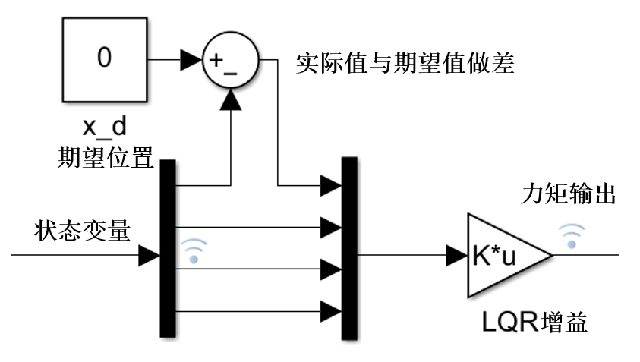
\includegraphics[width=0.65\linewidth]{figures/Sec4/lqrgram.png}
  \caption{
  实际仿真中,机器人采用的LQR控制器的示意图。
  }
  \label{fig:sec4-lqrgram}
   \vspace{6pt}
\end{figure}

为了实现鲁棒的平衡和轨迹跟踪,LQR\cite{li2012advanced}最优控制方法也被采用,并且用作和PID控制的对比。这里采用的式无穷水平线的固定反馈增益的LQR控制器,在给定状态变量惩罚矩阵$Q$和控制量惩罚矩阵$R$,最优的反馈控制增益$K$通过解如下的离散时间里卡蒂方程获得:
\begin{equation}
    P=A^TPA-(A^TPB)(R+B^TPB)^{-1}(B^TPA)+Q
    \label{eq:dare}
\end{equation}
我们已经获得了连续时间的状态空间方程,对其进行离散化之后,最优控制率可以用如下方式直接算出:
\begin{equation}
    K^* = (R+B^TPB)^{-1}B^TPA
    \label{eq:dare_sol}
\end{equation}

实际在仿真实验中,LQR控制器如图\ref{fig:sec4-lqrgram}所示。

\subsection{本章小结}

本章首先介绍了机器人的运动学和动力学模型,分别用在机器人的变高度控制和平衡控制,其中动力学模型进一步推导了状态空间方程。控制部分,首先介绍了简单的PID平衡及轨迹跟踪控制器,然后介绍了根据动力学模型确定的LQR最优控制器。
\clearpage
% !Mode:: "TeX:UTF-8"
% !TEX program  = xelatex
% \section{\LaTeX\ 入门}
% 请参考 \href{https://tex.readthedocs.io/zh_CN/latest/}{在线文档},包括学习资源及学习路径。欢迎在 GitHub 上提出 \href{https://github.com/Iydon/tex/issues}{Issues}。
\section{实验}

\subsection{引言}
对于实验部分,首先本设计建立了与CAD模型相对应的仿真模型,然后在仿真模型上测试控制算法。而在进行实验之前,须进行相关的硬件准备,如系统集成和参数辨识,然后再将仿真中测试成功的控制算法转移到实物模型上。如前文所说,仿真器选用的是MATLAB Simulink,可以快速实现仿真到实物的迁移。而系统集成主要是侧重于将已经搭建好的电气系统使用状态机搭建抽象的通讯网络,以实现初始化和保证机器人在运行时的安全性。如前文建模控制部分所言,由于机器人所有可活动杆件都被视为质心以计算整体小车-倒立摆模型的转动惯量,因此参数辨识主要侧重与获取机器人重心,而非各杆件的转动惯量。

\subsection{仿真模型}
仿真选择MATLAB Simulink Simscapes,从而可以实现仿真与实物的快速迁移。此外,作为商业引擎,Simulink Simscapes提供了精准的仿真和接触力模型,从而获得更好的仿真效果。在本论文中,仿真模型对CAD模型和实物进行了一定程度的简化。考虑到前文机械设计的部分提到的平行四边形连杆机构,其活动的连杆相对于大腿的运动幅度不大,且该连杆的质量也较小,因此可以将之视为与大腿固连的连杆,从而在运动学上实现了远端驱动的等效,在动力学上实现了远端驱动的简化。

\begin{figure}[h!]
  \centering
  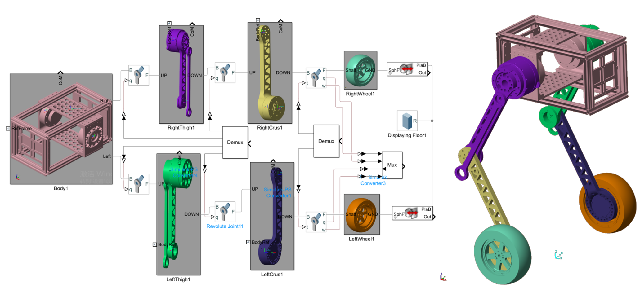
\includegraphics[width=1.0\linewidth]{figures/Sec5/simumod.png}
  \caption{
  左图:仿真模型搭建截图。右图:在Simulink可视化显示中的仿真3D模型。
  }
  \label{fig:sec5-simumod}
   \vspace{6pt}
\end{figure}


对于具体在仿真系统搭建模型,首先在CAD中导出每个零部件的通用3D文件(如STEP文件),然后分别导入仿真器,再每个零部件上根据实际情况定义坐标系,然后在坐标系之间定义位姿变换和运动副。这些零件和它们的坐标系被封装在一个子系统中,并且被增加了坐标系和零件的截图做的蒙版以方便区分,其与在MATLAB Simulink中仿真可视化界面展示的结果如图\ref{fig:sec5-simumod}所示,而其封装后,与控制器等如图\ref{fig:sec5-simuabs}所示。值得注意的是,上述部件使用转动副连接是针对机器人本身,而机器人与地面的交互则通过接触力模型来实现。根据理想机器人假设,机器人与地面的接触被认为是球-面接触,且机器人仅能沿轮子前后反向运动,而不能沿左右方向运动,满足非完整约束方程。但需要开始仿真,则需要定义机器人与世界系之间的虚拟6自由度关节,并给定初始条件。


\begin{figure}
  \centering
  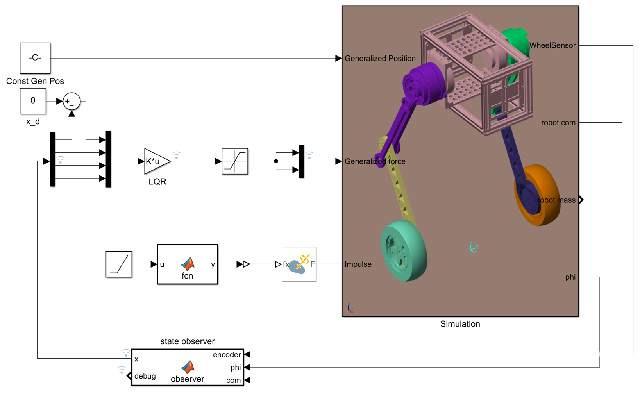
\includegraphics[width=0.85\linewidth]{figures/Sec5/simuabs.png}
  \caption{
  仿真封装示意图,其中右半部分被封装起来的部分是仿真器本身,接受位置和力指令,反馈机器人的状态。在本图中,使用了一个LQR控制器以同时实现平衡和轨迹跟踪。
  }
  \label{fig:sec5-simuabs}
   \vspace{6pt}
\end{figure}

\subsection{仿真实验}
在仿真实验中,主要实验目的是测试静态平衡,具体包括初始从一个非平衡的角度恢复至平衡状态,和受到外力扰动下重新回复到稳定状态的实现。在此基础上,测试矢状面的轨迹跟踪,具体为给定目标位置,机器人前往目标位置。如图\ref{fig:sec5-simuabs}所示,这里展示的是使用LQR控制器实现上述轨迹跟踪。使用针对轮子编码器进行加权和饱和的PID控制可以达到类似的效果。考虑到封装了仿真模型,因此上述控制器的切换较为简单。实际上仿真也实现了矢状面的轨迹跟踪,通过Simulink自带的滑块组件改变需要跟踪的位置值,即可实现机器人的轨迹跟踪。考虑到论文难以展示视频,因此主要集中在展示倾角恢复和抗扰两个方面。首先是倾角恢复,如图\ref{fig:sec5-lqr1}所示,机器人初始的质心与重锤线有0.1弧度(约6角度)的偏差,然后机器人在3秒的时间恢复平衡,并同时回到了原点的位置。而受到外界扰动恢复的实验中,如图\ref{fig:sec5-lqr2}所示,机器人首先在平衡状态下,当仿真时间在2s时,机器人受到大小为2Ns的冲量,随后在仿真时间5s时恢复平衡,且也恢复到原先的平衡点。仿真实验表明,使用先前章节所介绍的LQR控制器,起到了较好的平衡效果。可以看到当受到外力扰动时,机器人瞬间获得了角速度,然后通过加速移动改变质心位置,从而使用重力矩产生的冲量抵消外力产生的冲量。然后机器人的LQR控制器寻找到恢复到原先所在平衡点的路线,从而在角度和位移上恢复了原先的状态。

\begin{figure}
  \centering
  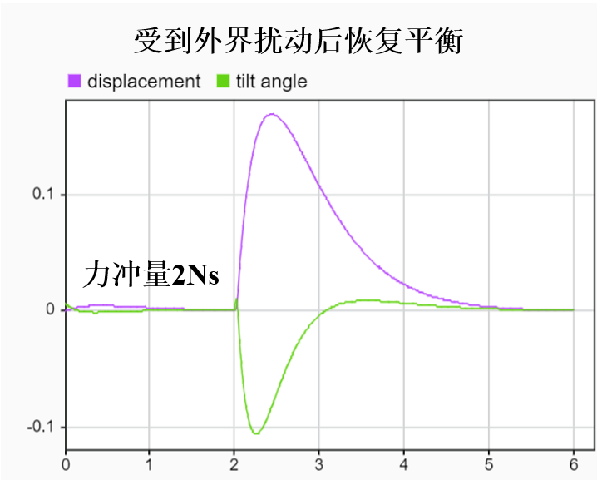
\includegraphics[width=0.6\linewidth]{figures/Sec5/lqr1.png}
  \caption{
  倾角恢复实验。机器人初始的质心与重锤线有0.1弧度(约6角度)的偏差,然后机器人在3秒的时间恢复平衡,并同时回到了原点的位置。
  }
  \label{fig:sec5-lqr1}
   \vspace{6pt}
\end{figure}

\begin{figure}[h]
  \centering
  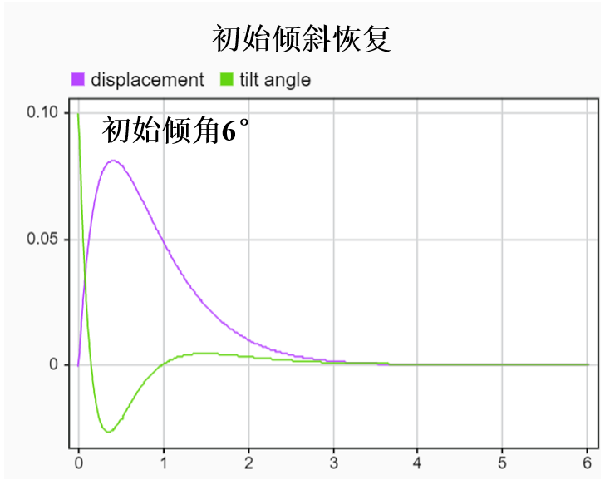
\includegraphics[width=0.6\linewidth]{figures/Sec5/lqr2.png}
  \caption{
  受到外界扰动恢复实验。机器人首先在平衡状态下,当仿真时间在2s时,机器人受到大小为2Ns的冲量,随后在仿真时间5s时恢复平衡,且也恢复到原先的平衡点。
  }
  \label{fig:sec5-lqr2}
   \vspace{6pt}
\end{figure}

\subsection{硬件准备}
如第二章所述,电气系统和控制系统的硬件上拥有2组不同的抽象控制网络,并且需要内置位置限制、电机使能和静能逻辑、电流限制和软件急停,因此需在再SpeedGoat内设计控制状态机,作为机器人控制器的底层保障系统。第二层系统反馈数据网络已由Simulink EtherCAT包封装好。另外如第四章所述,实物需要重新测定质心,因此采用了悬线测量法,通过IMU读取悬空静止角度得出重力方向,从而通过不同铅垂线交点获得质心位置。

\subsubsection{系统集成}
状态机主要包括以下几种状态。初始化进入状态,此时电机等待使能命令。使能状态,如前文所述,电机使能需要多次读取控制器STATUS WORD并发送CMD WORD,因此在获得遥控器的使能指令之后,所有电机会并行执行上述使能指令,并且根据驱动器反馈使能是否成功决定重新使能或进入下一个状态。下一个状态是等待新的位置指令状态,考虑到膝盖和胯部电机均工作在位置模式下,因此在使能之后,只有移动位置控制器才会激活膝盖电机和胯部电机的移动,以防止使能状态与位置滑块停留所代表的位置相差过大,误发送位置指令的情况。获得了新的位置指令之后,电机会进入执行位置指令的模式,并直到执行完之后,不接受新的位置指令。考虑到驱动器内建的位置模式刚性较大,因此实际上位置模式的实现是通过微小的位移量叠加而成。在将来的工作中,也可以设计成使用梯形曲线进行运动规划,从而可以在运动的过程中途改变目标位置。值得注意的是,轮子电机工作在扭矩或速度模式下,取决了控制器是LQR还是PID。但实际上在上述的四个状态中,在所有电机完成使能之后,平衡控制器就会自动开启,从而实现平衡和轨迹跟踪的功能。状态机的设计如图\ref{fig:sec5-stateflow}所示。值得注意的是,在任意状态下,接收到静能或软件急停指令时,状态机都会跳转到等待使能的状态并关闭迪纳基输出。而在位置跟踪的过程中,状态机会保证位置不会超过机械限位,同时会监看电流大小。当电流过大时,会退出位置跟踪状态并进入等待位置跟踪状态,以停止电流继续增大。

\begin{figure}
  \centering
  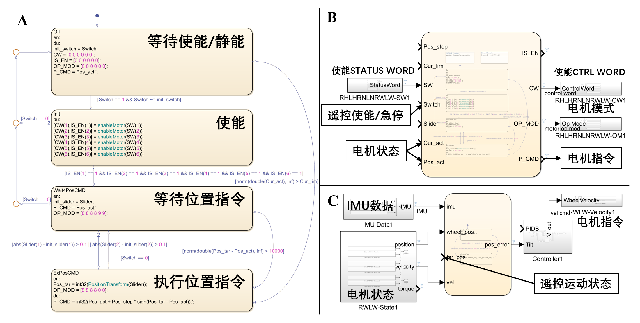
\includegraphics[width=1.0\linewidth]{figures/Sec5/stateflow.png}
  \caption{
  状态机示意图。其中左边的是状态机的四种状态。右边展示了状态机封装后的效果,左右分别是其输入和输出变量,用于和Simulink的其他模块交互。
  }
  \label{fig:sec5-stateflow}
   \vspace{6pt}
\end{figure}

\subsubsection{参数辨识}

\begin{figure}[h!]
  \centering
  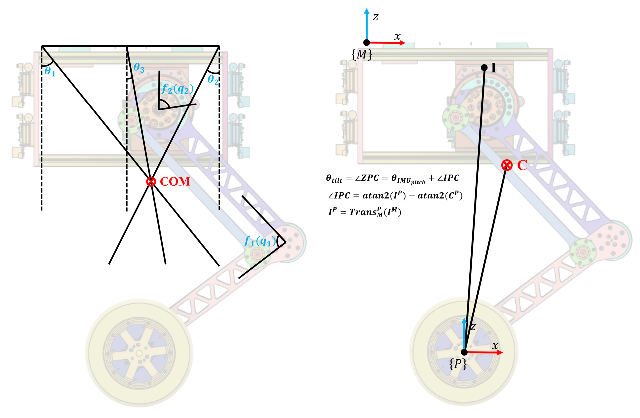
\includegraphics[width=0.85\linewidth]{figures/Sec5/comdata.png}
  \caption{
  质心测量示意图。根据这些几何关系,可以求出特定坐标系下的质心位置,从而通过最小二乘计算每个杆件在矢状面的质心位置。
  }
  \label{fig:sec5-comdata}
   \vspace{6pt}
\end{figure}

考虑到CAD模型与实际机器人在质心分布上有较大差异,如电机质量分布、轴承、螺丝、电线未计算在内,因此需要测定每个杆件的质心。传统上质心的测量方法是线悬法,但这里因为需要测量三维空间的质心,难度较大,且电线、轴承、螺丝等拆卸则无测定意义,因此会将整个机器人视作一个整体测定,而通过多组数据最小二乘计算出每个杆件的质心。考虑到目前机器人左右腿变高度是同步的,因此仅需要测定每个杆件在矢状面中的质心。如前文所述,根据机器人的运动学,假设每个杆件的质心位置为某变量后,可以计算出带变量的整体质心位置。

拥有多组数据后,便可以通过求解过约束线性方程组(最小二乘)实现质心的计算。虽然机器人质心可以通过在相同的构型下进行多次悬挂,同样针对质心位置计算另一次最小二乘,但实际上通过多组实验也可以实现减少误差的效果,因此在机器人已知位置设置两个悬挂点,然后在每个悬挂点悬挂时,改变机器人的构型,通过IMU记录重力方向,对第二个悬挂点也采用相同的方式。在采集了机器人构型数据和对应的IMU数据之后,在相同构型下, 通过重力方向可以计算出质心位置,计算方式如图\ref{fig:sec5-comdata}所示。值得注意的是,考虑到左右腿的同步性,其质量应当计算为原本2倍以得到正确的质心位置结果。


\subsection{实物实验}

\begin{figure}[h!]
  \centering
  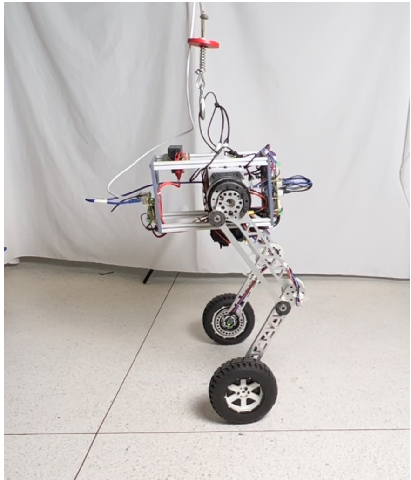
\includegraphics[width=0.45\linewidth]{figures/Sec5/simplerealresult.png}
  \caption{
  基于PID的实物静态平衡实验结果。可以看到其安全绳处于松弛状态,依靠平衡控制器实现了平衡。
  }
  \label{fig:sec5-simplerealresult}
   \vspace{6pt}
\end{figure}

基于上述内容,实物实验主要是将仿真实验转移到实物上。对于仿真模型,其质心位置根据仿真器的配置文件,通过机器人构型计算出,而实物则由测定的数据和机器人构型计算出,因此对于控制器而言,这个数据是“隐形”的,因为控制器仅需指导质心位置与竖直线间夹角即可。实物实验同样包括静态平衡和轨迹跟踪,在目前采用叠加位置跟踪的PID控制器与开环差速转向的情况下,其中平衡的效果如图\ref{fig:sec5-simplerealresult}所示,可以看到其安全绳出于松弛状态,依靠平衡控制器实现了平衡。此外,图\ref{fig:sec5-static}展示了其在延时摄影下的的平衡状态,可见机器人会以极慢的速度在极小范围内振荡,考虑到机器人实物原型机与控制模型的若干误差,可以认为机器人实际上已经达到平衡状态。

\begin{figure}[h!]
  \centering
  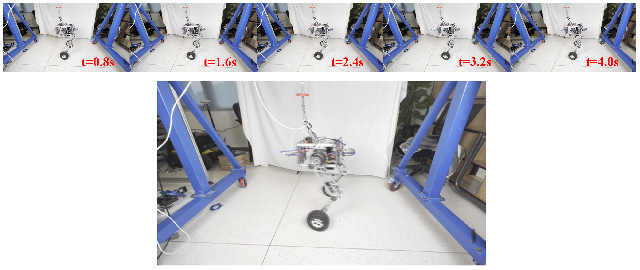
\includegraphics[width=1.0\linewidth]{figures/Sec5/static.png}
  \caption{
  基于PID的实物静态平衡实验结果。上图是平衡视频关键帧截图,下图是将关键帧叠加展示。
  }
  \label{fig:sec5-static}
   \vspace{6pt}
\end{figure}

\begin{figure}[h!]
  \centering
  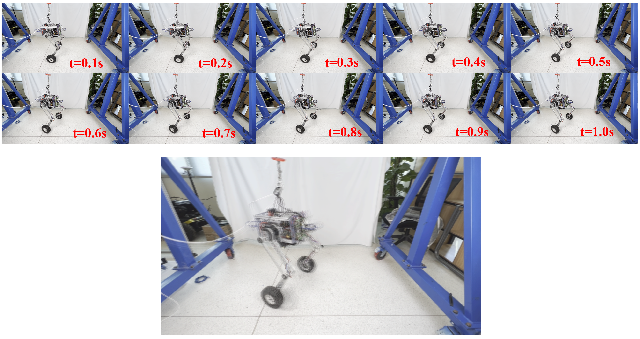
\includegraphics[width=1.0\linewidth]{figures/Sec5/rot.png}
  \caption{
  基于叠加位置跟踪的PID控制器与开环差速转向的实物原地自转的实验结果。上图是视频关键帧截图,下图是将关键帧叠加展示。
  }
  \label{fig:sec5-rot}
   \vspace{6pt}
\end{figure}

同样的,该控制器也实现了机器人在空间中的轨迹跟踪。为方便具体实现,给定轨迹为机器人质心处的定高度轨迹。据此,可以计算出每时刻机器人的质心速度,而考虑到机器人驱动轮为2自由度,因此需要根据若干时间窗口内的速度计算出机器人整体(此时机器人视为单一刚体)的角速度,则根据移动机器人的运动学方程(公式\ref{eq:naveq}),可以用于产生相应角速度的每轮线速度差速。这里不采用移动机器人运动学方程直接计算出每个轮子的速度,是考虑到欠驱动机器人,尤其是本轮腿机器人,最优先考虑的是平衡,因此具体的质心线速度和机器人角速度的实现分别需要融合在平衡控制器中,而不能单独实现。如图\ref{fig:sec4-3dsimple}和图\ref{fig:sec4-3dpid}所示的控制器可以实现线速度和角速度的闭环和开环控制。值得注意的是,机器人的线速度追踪采用对机器人在矢状面上位置点跟踪的方式实现,因此在输入控制器之前需要进行积分,这样设计的目的是使机器人不至于维持一个恒定的加速度平衡,或在受到外力扰动后可以获得一个返回原位置的趋势。而差速转向是开环控制,因此实际上机器人在实现轨迹跟踪时,仍需要一个更高层的控制器实现轨迹跟踪的反馈。考虑到机器人在非结构化的环境中活动且可能随时受到外界扰动,因此参考文献\cite{klemm2019ascento}中所述,将这个更高层的控制器认为是路径规划中的一部分,相应的本轮腿机器人则可以接受实时的、片段的轨迹,而不需要事先接受所有轨迹。


\begin{figure}[h]
  \centering
  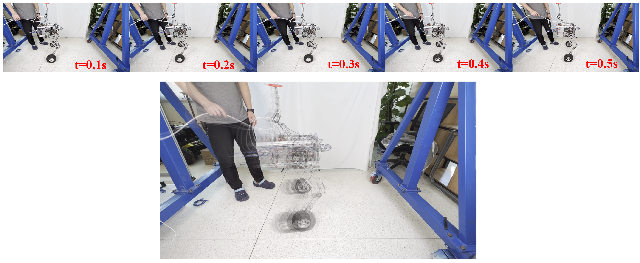
\includegraphics[width=1.0\linewidth]{figures/Sec5/movfd.png}
  \caption{
  基于叠加位置跟踪的PID控制器与开环差速转向的实物直线前进的实验结果。上图是视频关键帧截图,下图是将关键帧叠加展示。
  }
  \label{fig:sec5-movfd}
   \vspace{6pt}
\end{figure}


实际实验中,考虑安全性,机器人被安全绳限制在一定的活动范围内,且如上文所论述,实验主要测试机器人实现定速自转与定速直线运动。图\ref{fig:sec5-rot}是定速自转的截图,分别包括视频关键帧截图(每间隔0.1s为1关键帧),与关键帧叠加展示。考虑到实验条件,机器人自转速度较慢,但可通过第一张与最后一张关键帧明显看出机器人转动了约$\frac{\pi}{4} rad$,证明该控制器可以在保持平衡的状态下实现定速自转。

图\ref{fig:sec5-movfd}是则展示了定速直线运动的截图,也分别包括视频关键帧截图(每间隔0.1s为1关键帧),与关键帧叠加展示。通过关键帧的叠加显示可以明显看出机器人实现了定速直线运动,证明该控制器可以在保持平衡的状态下实现定速直线运动。

\subsection{本章小结}

在本章中,首先介绍了用于验证算法的仿真模型的搭建,以及之前章节中提到的算法在仿真模型上的验证。然后介绍了为原型机实验所做的准备,包括机器人的参数辨识与机电系统的集成。最后介绍了实物实验的具体设置、控制器,并分析了实验结果。\clearpage
\section{结论}
  本毕业设计主要设计并制作了一种二轮轮腿机器人,并建立了简化的数学模型,搭建了仿真模型,设计了控制算法并在仿真中进行测试,然后再实物原型机上机型实验。本轮腿机器人拥有6个自由度,其机械设计可靠稳定,电气系统高性能且易于开发,负载较大,可在后期加装感知机机械臂或用于辅助增强稳定性的动力尾或者涵道发动机。本轮腿机器人所有电机均为准直驱电机,可以实现力控,当前采用PID或者LQR实现轨迹跟踪,后期可结合动力尾、机械臂实现全身控制算法。本轮腿控制系统采用SpeedGoat控制器,使用MATLAB Simulink编程,与仿真环境一致,可以实现快速的控制算法实现-仿真测试-实物测试。仿真和实物实验显示,本轮腿的机械、电气和控制系统稳定可靠,且实现空间轨迹跟踪功能,为后续加装其他负载或实现全身力控算法打下坚实基础。 
  
  本毕业设计的机械设计部分主要采用CNC加工,后续可以考虑采用拓扑优化或衍生式设计,采用尼龙或金属3D打印加工实现。电机和驱动器的走线目前依然采用一端焊接连接,另一端使用接线柱连接的方式,集成度较低,且不利于安装,后续可以考虑设计功率PCB与EtherCAT通讯PCB连接,增强可维护性。为了实现所有关节的力控,膝盖电机和胯部电机也需要进行扭矩电流标定。且若机器人需要实现左右不同高度,则需要测量杆件在三维空间中的质心位置,因此需要采用单线悬吊法,解更加复杂的线性方程组获取质心位置。
  控制器方面,全身控制和转弯时的ZMP控制可以在MATLAB中快速设计,然后再仿真中验证,快速迁移到实物上。另外,躯干可以增加机械臂、动力尾或者喷气涵道,以增加稳定裕度和整体控制的简便程度,获得更好的控制效果。
  
  在实验方面,可以将龙门吊换成便于移动的铝合金吊架,从而可以在更大范围内测试机器人的轨迹跟踪性能,后期也可以在机器人上加装用于保护的碳纤维管,从而无需使用龙门吊限制机器人的运动范围,达到更好的实验效果。
  
  进一步地,可以考虑更换性能更好的电机驱动器,通过控制器插值实现变高度平衡算法,并探索研究跳跃,以及更高级的控制算法。\clearpage
\end{spacing}
\参考文献
  \def\bibfont{\fontsize{10.5}{18}\selectfont}
  \printbibliography[heading=none]\clearpage
\附录
  % !Mode:: "TeX:UTF-8"
% !TEX program  = xelatex
% \section*{数据获取函数}\label{A:data}
% \Python{utils.py}{code/examples/utils.py}

% \section*{机器人物料表}


% \clearpage
\section*{部分零件机械设计图纸}

\begin{figure}[h!]
  \centering
  \includegraphics[width=1.4\linewidth, angle=90]{figures/appendix/dwg1.pdf}
   \vspace{6pt}
\end{figure}

\begin{figure}
  \centering
  \includegraphics[width=1.4\linewidth, angle=90]{figures/appendix/dwg2.pdf}
   \vspace{6pt}
\end{figure}

\begin{figure}
  \centering
  \includegraphics[width=1.4\linewidth, angle=90]{figures/appendix/dwg3.pdf}
   \vspace{6pt}
\end{figure}

\begin{figure}
  \centering
  \includegraphics[width=1.4\linewidth, angle=90]{figures/appendix/dwg4.pdf}
   \vspace{6pt}
\end{figure}

\begin{figure}
  \centering
  \includegraphics[width=1.4\linewidth, angle=90]{figures/appendix/dwg5.pdf}
   \vspace{6pt}
\end{figure}

\begin{figure}
  \centering
  \includegraphics[width=1.4\linewidth, angle=90]{figures/appendix/dwg6.pdf}
   \vspace{6pt}
\end{figure}

\begin{figure}
  \centering
  \includegraphics[width=1.4\linewidth, angle=90]{figures/appendix/dwg7.pdf}
   \vspace{6pt}
\end{figure}

\begin{figure}
  \centering
  \includegraphics[width=1.4\linewidth, angle=90]{figures/appendix/dwg8.pdf}
   \vspace{6pt}
\end{figure}

\begin{figure}
  \centering
  \includegraphics[width=1.4\linewidth, angle=90]{figures/appendix/dwg9.pdf}
   \vspace{6pt}
\end{figure}

\begin{figure}
  \centering
  \includegraphics[width=1.4\linewidth, angle=90]{figures/appendix/dwg10.pdf}
   \vspace{6pt}
\end{figure}

\begin{figure}
  \centering
  \includegraphics[width=1.4\linewidth, angle=90]{figures/appendix/dwg11.pdf}
   \vspace{6pt}
\end{figure}

\clearpage

\section*{部分3D打印件示意图}

\begin{figure}[h!]
  \centering
  \includegraphics[width=1.4\linewidth, angle=90]{figures/appendix/3d1.png}
   \vspace{6pt}
\end{figure}

\begin{figure}
  \centering
  \includegraphics[width=1.4\linewidth, angle=90]{figures/appendix/3d2.png}
   \vspace{6pt}
\end{figure}

\begin{figure}
  \centering
  \includegraphics[width=1.4\linewidth, angle=90]{figures/appendix/3d3.png}
   \vspace{6pt}
\end{figure}

\clearpage

% \section*{机器人运动学及动力学参数}


% \clearpage
% \section*{状态机控制代码}


% \clearpage
% \section*{仿真及实验控制器参数}


% \clearpage\clearpage
\致谢
  % !Mode:: "TeX:UTF-8"
% !TEX program  = xelatex
% \sustechthesis\ 目前版本为 \version, \LaTeX\ 毕业论文模板项目从提出到现在已有两年了。感谢为本项目贡献代码的开发人员们:
% \begin{itemize}
%     \item 梁钰栋(南方科技大学,本科 17 级);
%     \item 张志炅(南方科技大学,本科 17 级)。
% \end{itemize}
% 以及使用本项目,并提出诸多宝贵的修改意见的使用人员们:
% \begin{itemize}
%     \item 李未晏(南方科技大学,本科 15 级);
%     \item 张尔聪(南方科技大学,本科 15 级)。
% \end{itemize}

% 此外,目前的维护者并非计算机系,可能存在对协议等的错误使用,如果你在本模板中发现任何问题,请在 GitHub 中提出 \href{https://github.com/Iydon/sustechthesis/issues}{Issues},同时也非常欢迎对代码的贡献!

衷心感谢贾振中助理教授、朱政研究副教授对本人的精心指导。老师们经常与我讨论宏观的研究方法与具体的技术细节,为课题点明了方向,他们的言传身教将使我终生受益。

在课题研究过程中,林世远师兄和朱政研究副教授对我帮助良多,本毕业设计使用的电机、电机驱动及和IMU等均是在他们的帮助下选型、调试,机械设计方面,许多都是和林世远师兄讨论确定的,IMU转EtherCAT、遥控器的PCB是在朱政研究副教授的帮助下打样的,机器人实物制作往往不是一帆风顺的,其中充满各种有挑战的工程问题,如果没有他们丰富的经验和的细心的指导,这个课题很难走到目前这一步。与我一同届的黄滨鑫同学帮助计算了轮腿杆件的一些机械参数,并辅助做了实验。

此外还要感谢实验是的师兄弟们,和支持我的朋友们,对课题的关心与建议。

作为本科生,能做出这样的毕业设计,作为本科生涯的圆满的句号,我充满喜悦与自豪,在此衷心感谢所有关心我的人。

愿大家都有光明美好的未来!
\clearpage
  
\在学期间完成的相关学术成果

\section*{发表的学术论文}

\begin{achievements}

    \item \textbf{Yuntian Zhao}, Shiyuan Lin, Zheng Zhu and Zhenzhong Jia. A Bipedal Wheel-Legged Robot with Improved Balancing and Disturbance Rejection Capability Assisted by Electrical-Jets. IEEE International Conference on Advanced Robotics and Mechatronics (ARM), 2022. 已接收.
    
    \item Shipeng Lv, \textbf{Yuntian Zhao}, Zhenyang Chen, Chengyuan Gao, Longteng Hu and Zhenzhong Jia. Improved Rover Mobility Over Loose Deformable Slopes through Active Control of Body-Rotating Mechanism. 2021 27th International Conference on Mechatronics and Machine Vision in Practice (M2VIP), 2021. 已发表.
    
    \item Shiyuan Lin, \textbf{Yuntian Zhao}, Zheng Zhu and Zhenzhong Jia. A Quasi-Direct Drive Hand for Contact-rich Manipulations. IEEE International Conference on Advanced Robotics and Mechatronics (ARM), 2022. 已接收.
    
    \item Chengyuan Gao, Zhuolun Li, \textbf{Yuntian Zhao}, Zheng Zhu and Zhenzhong Jia. Design of an scaled-car platform for extreme driving conditions. IEEE International Conference on Advanced Robotics and Mechatronics (ARM), 2022. 已接收.
    
\end{achievements}

\section*{大学生创新创业项目}

\begin{achievements}
  \item 用于斜坡攀爬穿越的变质心火星车的机理与实验研究,已结题,省级大学生创新创业项目,项目负责人.
  \item 四轮独立驱动高频力矩控制小车平台,已结题,校级大学生创新创业项目,项目成员.
\end{achievements}
  
 \section*{专利}

\begin{achievements}
  \item 一种基于QDD电机的轮腿机器人及其复合驱动平衡控制. 发明人:贾振中,\textbf{赵云天},林世远,朱政. 申请中.
\end{achievements}

 \section*{学科竞赛}

\begin{achievements}
  \item 中国大学生电动方程式赛车(FSEC)2018 年参赛队员.
  \item 2019 RoboMaster 机甲大师南部分区赛团体三等奖.
\end{achievements}

\end{document}
